% =========================================================
%  Rapport de mini projet Web — Mosaïque (FIA3, ISSAT Sousse)
%  Compilation : pdflatex rapport.tex (deux fois, pour le sommaire)
%  ou : latexmk -pdf rapport.tex
%  Sur Overleaf : mettre images/ et code/ (index.html, style.css) à côté de ce fichier
% =========================================================
\documentclass[12pt,a4paper]{article}

% ---------- Langue et encodage ----------
\usepackage[utf8]{inputenc}
\usepackage[T1]{fontenc}
\usepackage[french]{babel}
\usepackage{lmodern}

% ---------- Mise en page ----------
\usepackage[margin=2.5cm]{geometry}
\usepackage{graphicx}
\usepackage{float}
\usepackage{caption}
\usepackage{subcaption}
\usepackage{booktabs}
\usepackage{tabularx}
\usepackage{array}
\usepackage{enumitem}
\usepackage{pmboxdraw}  % caractères ├ └ │ de l'arborescence
\usepackage{xcolor}
\usepackage{titlesec}
\usepackage{fancyhdr}
\usepackage[hidelinks]{hyperref}
\usepackage{tcolorbox}
\tcbuselibrary{skins}
\usepackage{fontawesome5}   % icônes GitHub et globe

% ---------- Couleurs de la charte graphique ----------
\definecolor{encre}{HTML}{1A1A1A}
\definecolor{papier}{HTML}{FAF7F2}
\definecolor{terracotta}{HTML}{C0492B}
\definecolor{gris}{HTML}{6B6B6B}
\definecolor{bordure}{HTML}{E5E0D8}

% Titres de section en terracotta
\titleformat{\section}{\Large\bfseries\color{terracotta}}{\thesection.}{0.6em}{}
\titleformat{\subsection}{\large\bfseries\color{encre}}{\thesubsection}{0.6em}{}

% Pied de page : numéro de page
\pagestyle{fancy}
\fancyhf{}
\fancyfoot[R]{\thepage}
\fancyfoot[L]{\small\color{gris}Mosaïque — Rapport de mini projet Web}
\renewcommand{\headrulewidth}{0pt}

% Légendes des figures et tableaux
\captionsetup{font=small,labelfont=bf}

% ---------- Code source (listings) ----------
\usepackage{listings}
\lstset{
  basicstyle=\ttfamily\small,
  keywordstyle=\color{terracotta}\bfseries,
  commentstyle=\color{gris}\itshape,
  stringstyle=\color{encre},
  backgroundcolor=\color{papier},
  frame=l,
  framerule=2pt,
  rulecolor=\color{terracotta},
  xleftmargin=10pt,
  framexleftmargin=6pt,
  breaklines=true,
  columns=fullflexible,
  keepspaces=true,
  showstringspaces=false,
  tabsize=2,
  % Caractères accentués présents dans le code
  literate=
    {é}{{\'e}}1 {è}{{\`e}}1 {ê}{{\^e}}1 {à}{{\`a}}1 {ç}{{\c{c}}}1
    {ï}{{\"i}}1 {î}{{\^i}}1 {ô}{{\^o}}1 {É}{{\'E}}1 {À}{{\`A}}1
    {«}{{\guillemotleft}}1 {»}{{\guillemotright}}1 {—}{{---}}1
    {›}{{\guilsinglright}}1 {©}{{\textcopyright}}1
    {→}{{$\rightarrow$}}1 {←}{{$\leftarrow$}}1
}
\lstdefinelanguage{CSS}{
  morekeywords={display,grid,grid-template-columns,gap,overflow,transform,
    transition,flex,position,color,background-color,box-shadow,
    aspect-ratio,object-fit,@media,max-width,padding,margin,border},
  sensitive=true,
  morecomment=[s]{/*}{*/},
  morestring=[b]",
}
\lstdefinelanguage{HTML5}{
  language=HTML,
  morekeywords={header,nav,main,section,article,footer,figure,figcaption,
    time,label,input,button,ul,li,a,img,span,div,form,h1,h2,h3,p},
  sensitive=true,
  morecomment=[s]{<!--}{-->},
  morestring=[b]",
}

% Inclut un fichier de code du site : cherche d'abord dans code/ (projet
% Overleaf), puis dans le dépôt (../). Si le fichier manque, affiche une
% note au lieu d'arrêter la compilation.
\newcommand{\codefile}[3]{%
  \IfFileExists{code/#2}{\lstinputlisting[#1]{code/#2}}{%
    \IfFileExists{#3}{\lstinputlisting[#1]{#3}}{%
      \textit{Fichier \texttt{#2} introuvable : ajoutez-le dans le dossier
      \texttt{code/} du projet.}}}}

% ---------- Liens du projet (couleurs de la charte) ----------
% Petite étiquette en majuscules, comme les rubriques du site
\newcommand{\etiquette}[1]{{\footnotesize\bfseries\color{terracotta}\MakeUppercase{#1}}}
% Bouton terracotta, comme le bouton « S'abonner » du site
\newcommand{\bouton}[2]{%
  \tcbox[on line, colback=terracotta, colframe=terracotta, coltext=white,
    arc=0.6mm, boxrule=0pt, left=3mm, right=3mm, top=1.2mm, bottom=1.2mm]%
  {\href{#1}{\textbf{#2}}}}
% Carte d'un dépôt GitHub : étiquette, auteur, compte, nom du dépôt
\newcommand{\depot}[4]{%
  \begin{minipage}[t]{0.47\linewidth}
    \etiquette{\faGithub\ #1}\\[1mm]
    {\color{encre}\bfseries #2}\\[0.5mm]
    \href{https://github.com/#3/#4}{\footnotesize\color{gris}\ttfamily
      github.com/#3/\\#4}
  \end{minipage}}

% Raccourci pour les noms de code dans le texte
\newcommand{\code}[1]{\texttt{#1}}

% =========================================================
\begin{document}

% ---------------- Page de garde ----------------
\begin{titlepage}
  \thispagestyle{empty}
  \begin{minipage}[t]{0.48\textwidth}
    \centering\small
    République Tunisienne\\
    Ministère de l'Enseignement Supérieur\\
    et de la Recherche Scientifique\\
    Université de Sousse
  \end{minipage}\hfill
  \begin{minipage}[t]{0.48\textwidth}
    \centering\small
    Institut Supérieur des Sciences\\
    Appliquées et de Technologie\\
    de Sousse
  \end{minipage}

  \vspace{2.5cm}
  \begin{center}
    {\large\bfseries DÉPARTEMENT INFORMATIQUE}\\[2cm]
    {\LARGE\bfseries RAPPORT DE MINI PROJET WEB}\\[0.6cm]
    {\Large FIA3}\\[2cm]
    {\color{terracotta}\rule{0.6\textwidth}{1pt}}\\[0.5cm]
    {\Huge\bfseries Mosaïque}\\[0.3cm]
    {\Large Mini magazine en ligne}\\[0.3cm]
    {\color{terracotta}\rule{0.6\textwidth}{1pt}}
  \end{center}

  \vspace{2cm}
  \noindent\textbf{Élaboré par :}\\[0.3cm]
  \hspace*{4cm}Étudiante 1 : Ranim Boussama\\
  \hspace*{4cm}Étudiante 2 : Yasmine Mtawaa

  \vfill
  \noindent\textbf{A.U. :} 2025/2026
\end{titlepage}

% ---------------- Plan ----------------
\renewcommand{\contentsname}{Plan}
\tableofcontents
\newpage

% =========================================================
\section{Introduction}

Ce rapport présente \textbf{Mosaïque}, un mini magazine en ligne consacré
à la tech et au numérique, réalisé dans le cadre du module Web en FIA3 à
l'ISSAT Sousse.

Le sujet choisi est le Sujet 6, « Mini magazine en ligne ». Il consiste à
créer un site qui ressemble à un vrai magazine : une page d'accueil avec
une grille d'articles, des pages d'article et une navigation entre les
pages. Notre magazine traite de cinq rubriques : l'intelligence
artificielle, les gadgets, les jeux vidéo, la cybersécurité et le
développement web.

Le projet est construit en trois étapes, une technologie par semaine. La
semaine 1 porte sur la structure et la mise en forme avec HTML5 et CSS3
uniquement. La semaine 2 ajoutera JavaScript (interactivité, validation
des formulaires), puis la semaine 3 ajoutera PHP (traitement des
formulaires côté serveur). Chaque étape complète le code de la précédente,
sans repartir de zéro.

\medskip
\noindent\textit{Cette version du rapport couvre la semaine 1 (HTML et CSS).}

% =========================================================
\section{Cahier des charges / Objectifs}

L'objectif principal est de créer une interface de type magazine qui
présente plusieurs articles et de simuler la navigation entre les pages,
en respectant les contraintes techniques du sujet. Le site doit être
lisible et agréable sur ordinateur, tablette et téléphone, et son code
doit passer la validation du W3C. Le tableau~\ref{tab:exigences} montre
comment chaque exigence du sujet est traitée dans Mosaïque.

\begin{table}[H]
  \centering
  \small
  \begin{tabularx}{\textwidth}{>{\raggedright\arraybackslash}p{5cm}X}
    \toprule
    \textbf{Exigence du sujet} & \textbf{Réponse dans Mosaïque} \\
    \midrule
    HTML5 et CSS3 uniquement (semaine 1) &
      Aucune ligne de JavaScript ni de PHP ; le menu mobile et le menu
      déroulant fonctionnent en CSS pur \\
    Page d'accueil avec une grille de 6 à 9 articles &
      Un article à la une + une grille de 9 cartes construite avec CSS Grid \\
    Effet zoom au survol des images &
      \code{transform: scale(1.1)} sur l'image de chaque carte, avec une ombre \\
    Navigation simulée entre pages &
      Liens vers les pages article, rubrique et contact, fil d'Ariane et
      lien « Retour à l'accueil » \\
    Responsive design obligatoire &
      3 colonnes sur ordinateur, 2 sur tablette, 1 sur petit téléphone,
      grâce aux media queries \\
    Fichiers HTML et CSS séparés &
      Une seule feuille \code{css/style.css}, liée à toutes les pages \\
    Validation W3C du code &
      HTML et CSS vérifiés avec les validateurs du W3C \\
    \bottomrule
  \end{tabularx}
  \caption{Exigences du sujet et réponses apportées}
  \label{tab:exigences}
\end{table}

En plus de ces exigences, nous nous sommes fixé deux objectifs : une
identité visuelle soignée inspirée de la presse écrite, et un site
accessible (lien d'évitement, textes alternatifs, navigation au clavier).

% =========================================================
\section{Conception}

Avant d'écrire le code, nous avons défini l'organisation des fichiers, la
structure des pages et l'identité visuelle, puis dessiné les maquettes sur
Figma.

\subsection{Structure du dossier}

Le projet sépare clairement le contenu (HTML), la mise en forme (CSS) et
les médias (images). Toutes les pages utilisent la même feuille de style.

\begin{verbatim}
/mosaique
├── index.html                  (page d'accueil)
├── css/
│   └── style.css               (feuille de style unique)
├── images/
│   └── article-1.png ... article-10.png
└── pages/
    ├── article-1.html ... article-10.html
    ├── categorie-ia.html
    ├── categorie-gadgets.html
    ├── categorie-jeux.html
    ├── categorie-cyber.html
    ├── categorie-dev.html
    └── contact.html
\end{verbatim}

\subsection{Structure HTML}

Chaque page suit la même organisation logique, avec des balises
sémantiques HTML5 :

\begin{itemize}
  \item \code{<header>} : un bandeau noir avec la date et le slogan, le
    logo Mosaïque et le menu de navigation \code{<nav>} (Accueil,
    Catégories, Contact).
  \item \code{<main>} : le contenu propre à chaque page. Sur l'accueil, il
    contient l'article à la une, la liste des rubriques, la grille des
    derniers articles et l'encart newsletter.
  \item \code{<article>} : chaque carte de la grille est un article
    indépendant (image, rubrique, titre, résumé, auteur).
  \item \code{<footer>} : le logo, les liens vers les rubriques et les
    pages du magazine, et les mentions du projet.
\end{itemize}

Trois types de pages sont prévus : l'accueil, la page article et la page
rubrique, auxquelles s'ajoute la page contact.

\subsection{Charte graphique}

Nous avons choisi un style inspiré de la presse écrite : un fond couleur
papier, des titres à empattement et une seule couleur d'accent, le
terracotta.

\begin{table}[H]
  \centering
  \small
  \begin{tabular}{l l l l}
    \toprule
    & \textbf{Nom} & \textbf{Code} & \textbf{Utilisation} \\
    \midrule
    \fcolorbox{bordure}{encre}{\rule{0pt}{8pt}\rule{8pt}{0pt}} & Encre & \#1A1A1A & Titres, texte, bandeau et pied de page \\
    \fcolorbox{bordure}{papier}{\rule{0pt}{8pt}\rule{8pt}{0pt}} & Papier & \#FAF7F2 & Fond des pages \\
    \fcolorbox{bordure}{white}{\rule{0pt}{8pt}\rule{8pt}{0pt}} & Blanc & \#FFFFFF & Fond des cartes \\
    \fcolorbox{bordure}{terracotta}{\rule{0pt}{8pt}\rule{8pt}{0pt}} & Terracotta & \#C0492B & Accent : liens, rubriques, boutons \\
    \fcolorbox{bordure}{gris}{\rule{0pt}{8pt}\rule{8pt}{0pt}} & Gris & \#6B6B6B & Texte secondaire (résumés, auteurs) \\
    \fcolorbox{bordure}{bordure}{\rule{0pt}{8pt}\rule{8pt}{0pt}} & Bordure & \#E5E0D8 & Séparateurs et contours des cartes \\
    \bottomrule
  \end{tabular}
  \caption{Palette de couleurs de Mosaïque}
\end{table}

Pour la typographie, nous utilisons deux polices Google Fonts.
\textbf{Playfair Display} sert aux titres (h1 48px, h2 32px, h3 22px) et,
en italique, aux citations. \textbf{Inter} sert au texte courant (16px,
interligne 1,7) et aux étiquettes de rubrique (semi-gras, 12px,
majuscules, espacement 0,1em).

\begin{figure}[H]
  \centering
  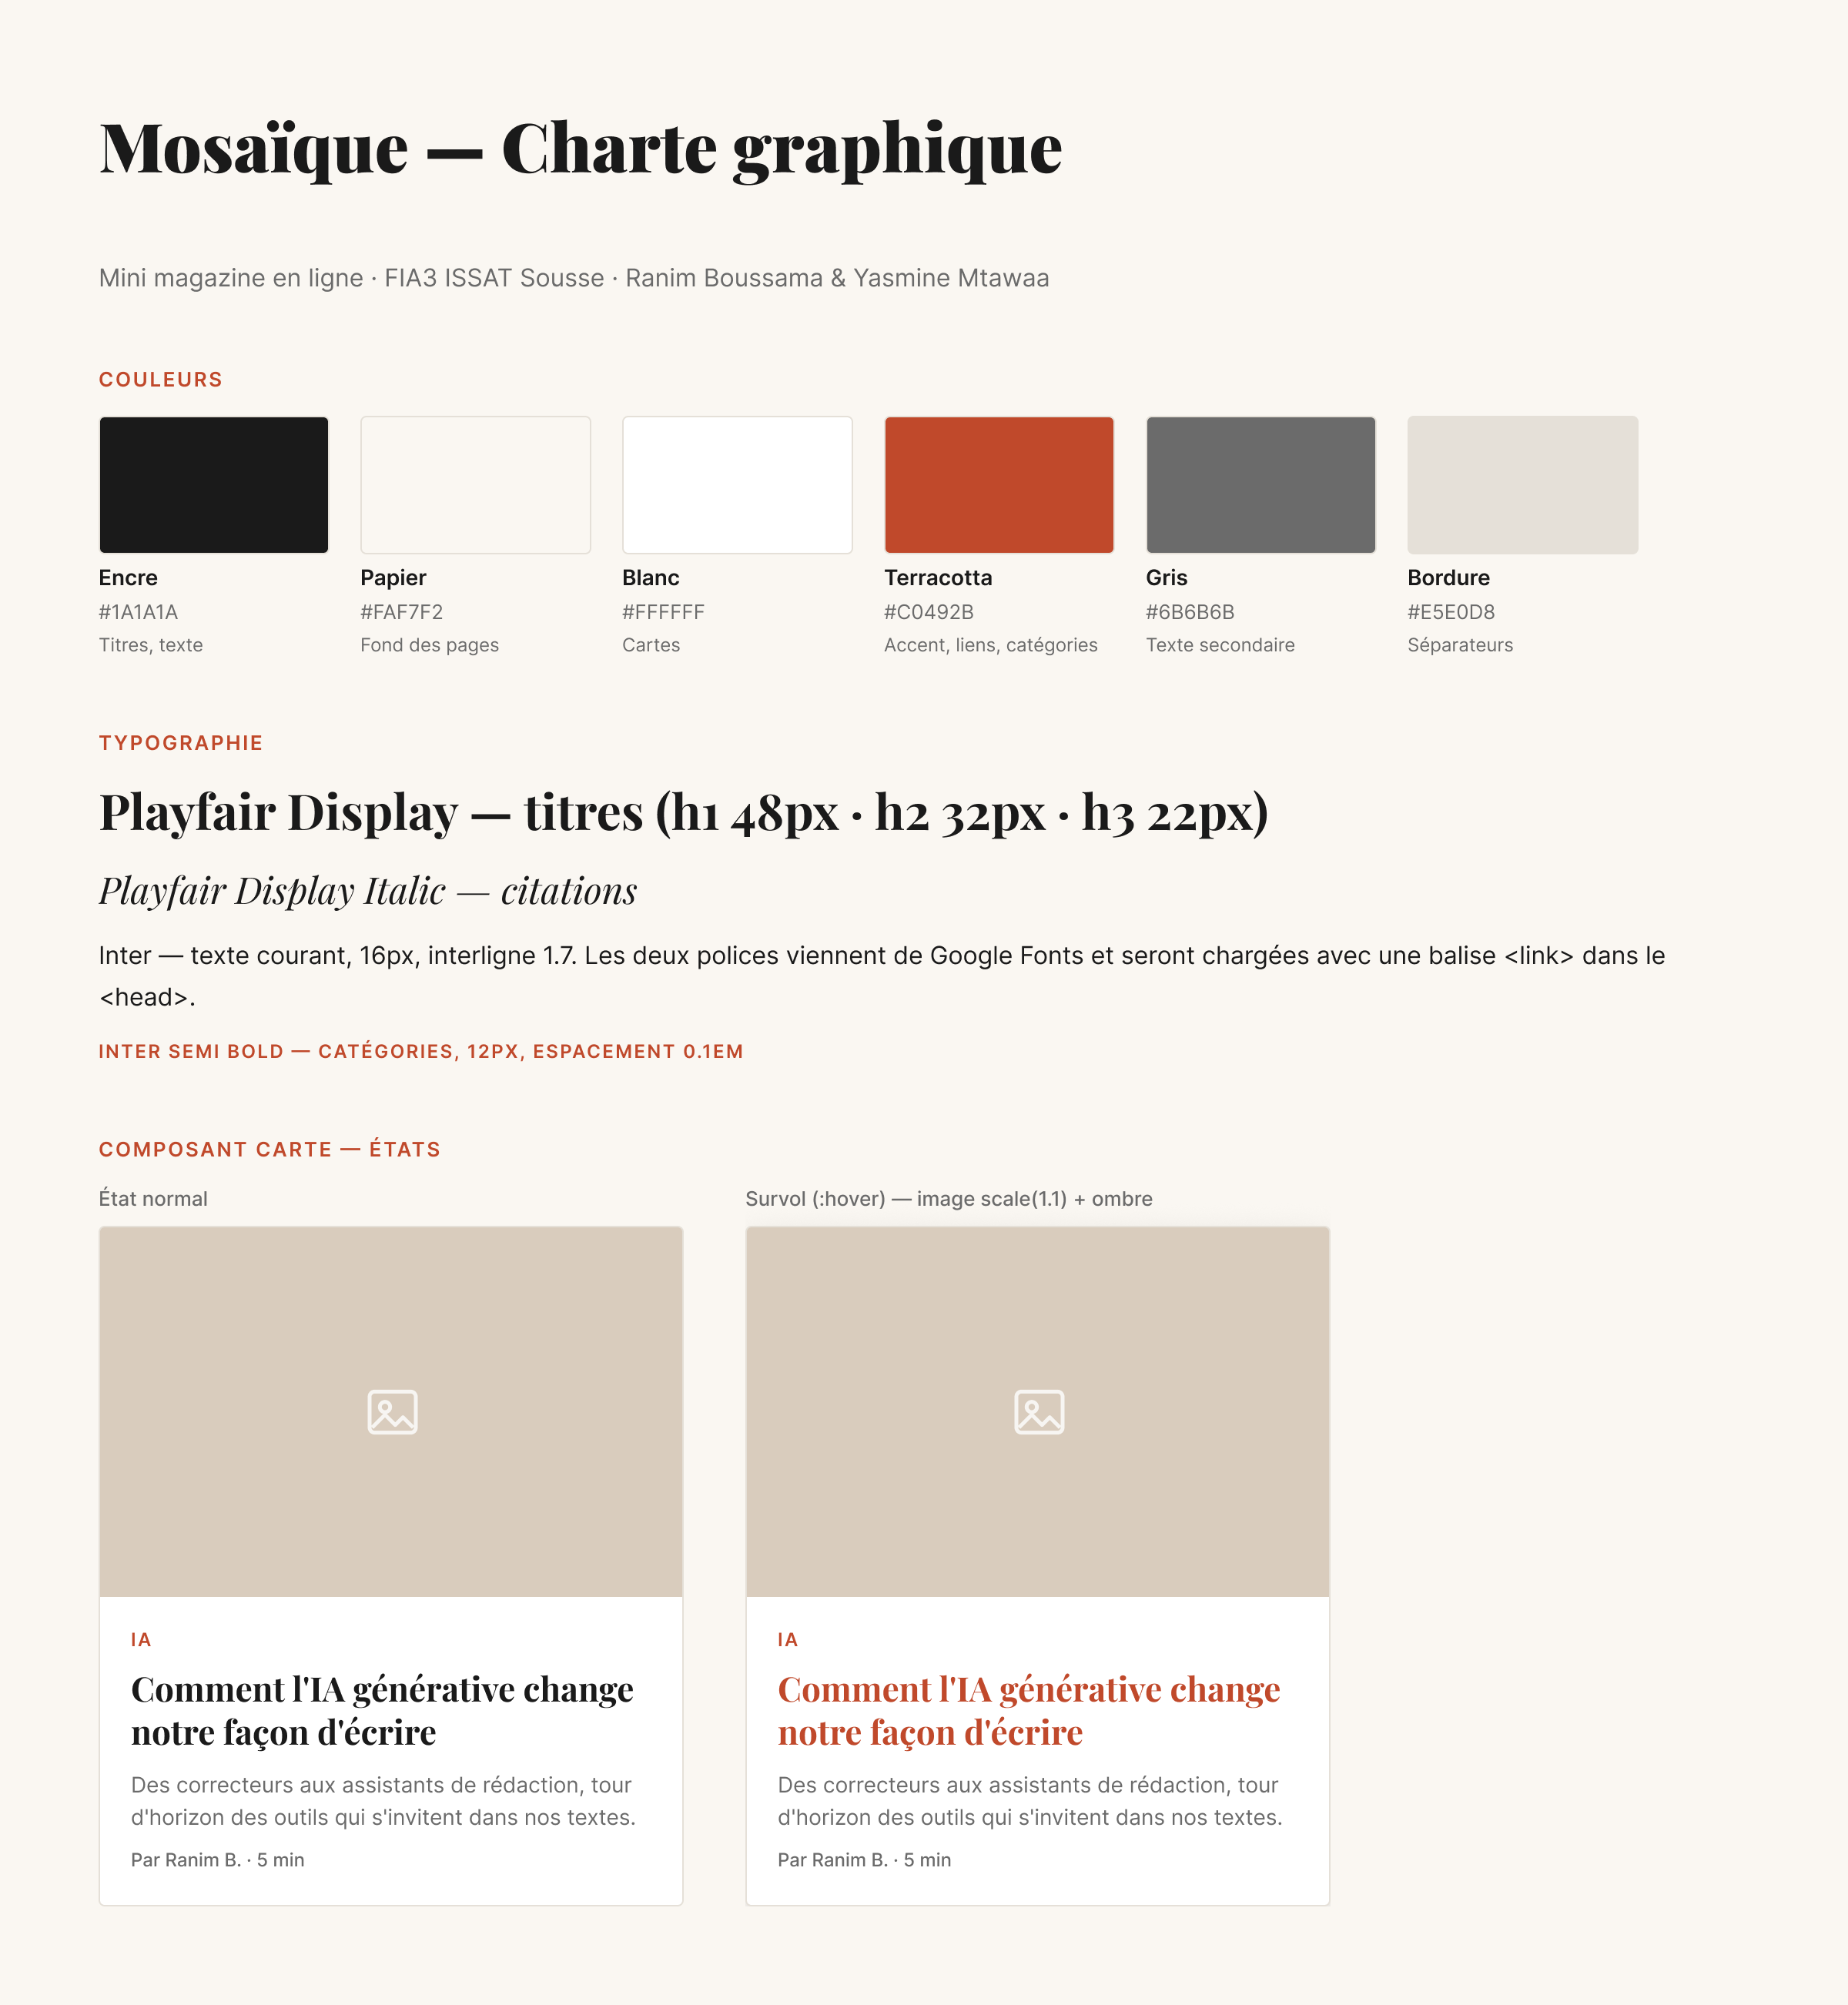
\includegraphics[width=0.8\textwidth]{images/charte-graphique.png}
  \caption{Charte graphique de Mosaïque (Figma) : couleurs, typographie et
    états de la carte article (normal et survol)}
\end{figure}

\subsection{Maquettes Figma}

Nous avons réalisé les maquettes desktop sur Figma avant de coder, avec
les vrais contenus du magazine : les cinq rubriques (IA, Gadgets, Jeux
vidéo, Cybersécurité, Dev web) et les titres des articles. Elles ont servi
de référence pour les dimensions, les espacements et la position de chaque
élément. Comme sur la maquette, le menu du site regroupe les cinq
rubriques dans un menu déroulant « Catégories », ce qui garde une barre de
navigation courte (Accueil, Catégories, Contact).

\begin{figure}[H]
  \centering
  \begin{subfigure}[t]{0.45\textwidth}
    \centering
    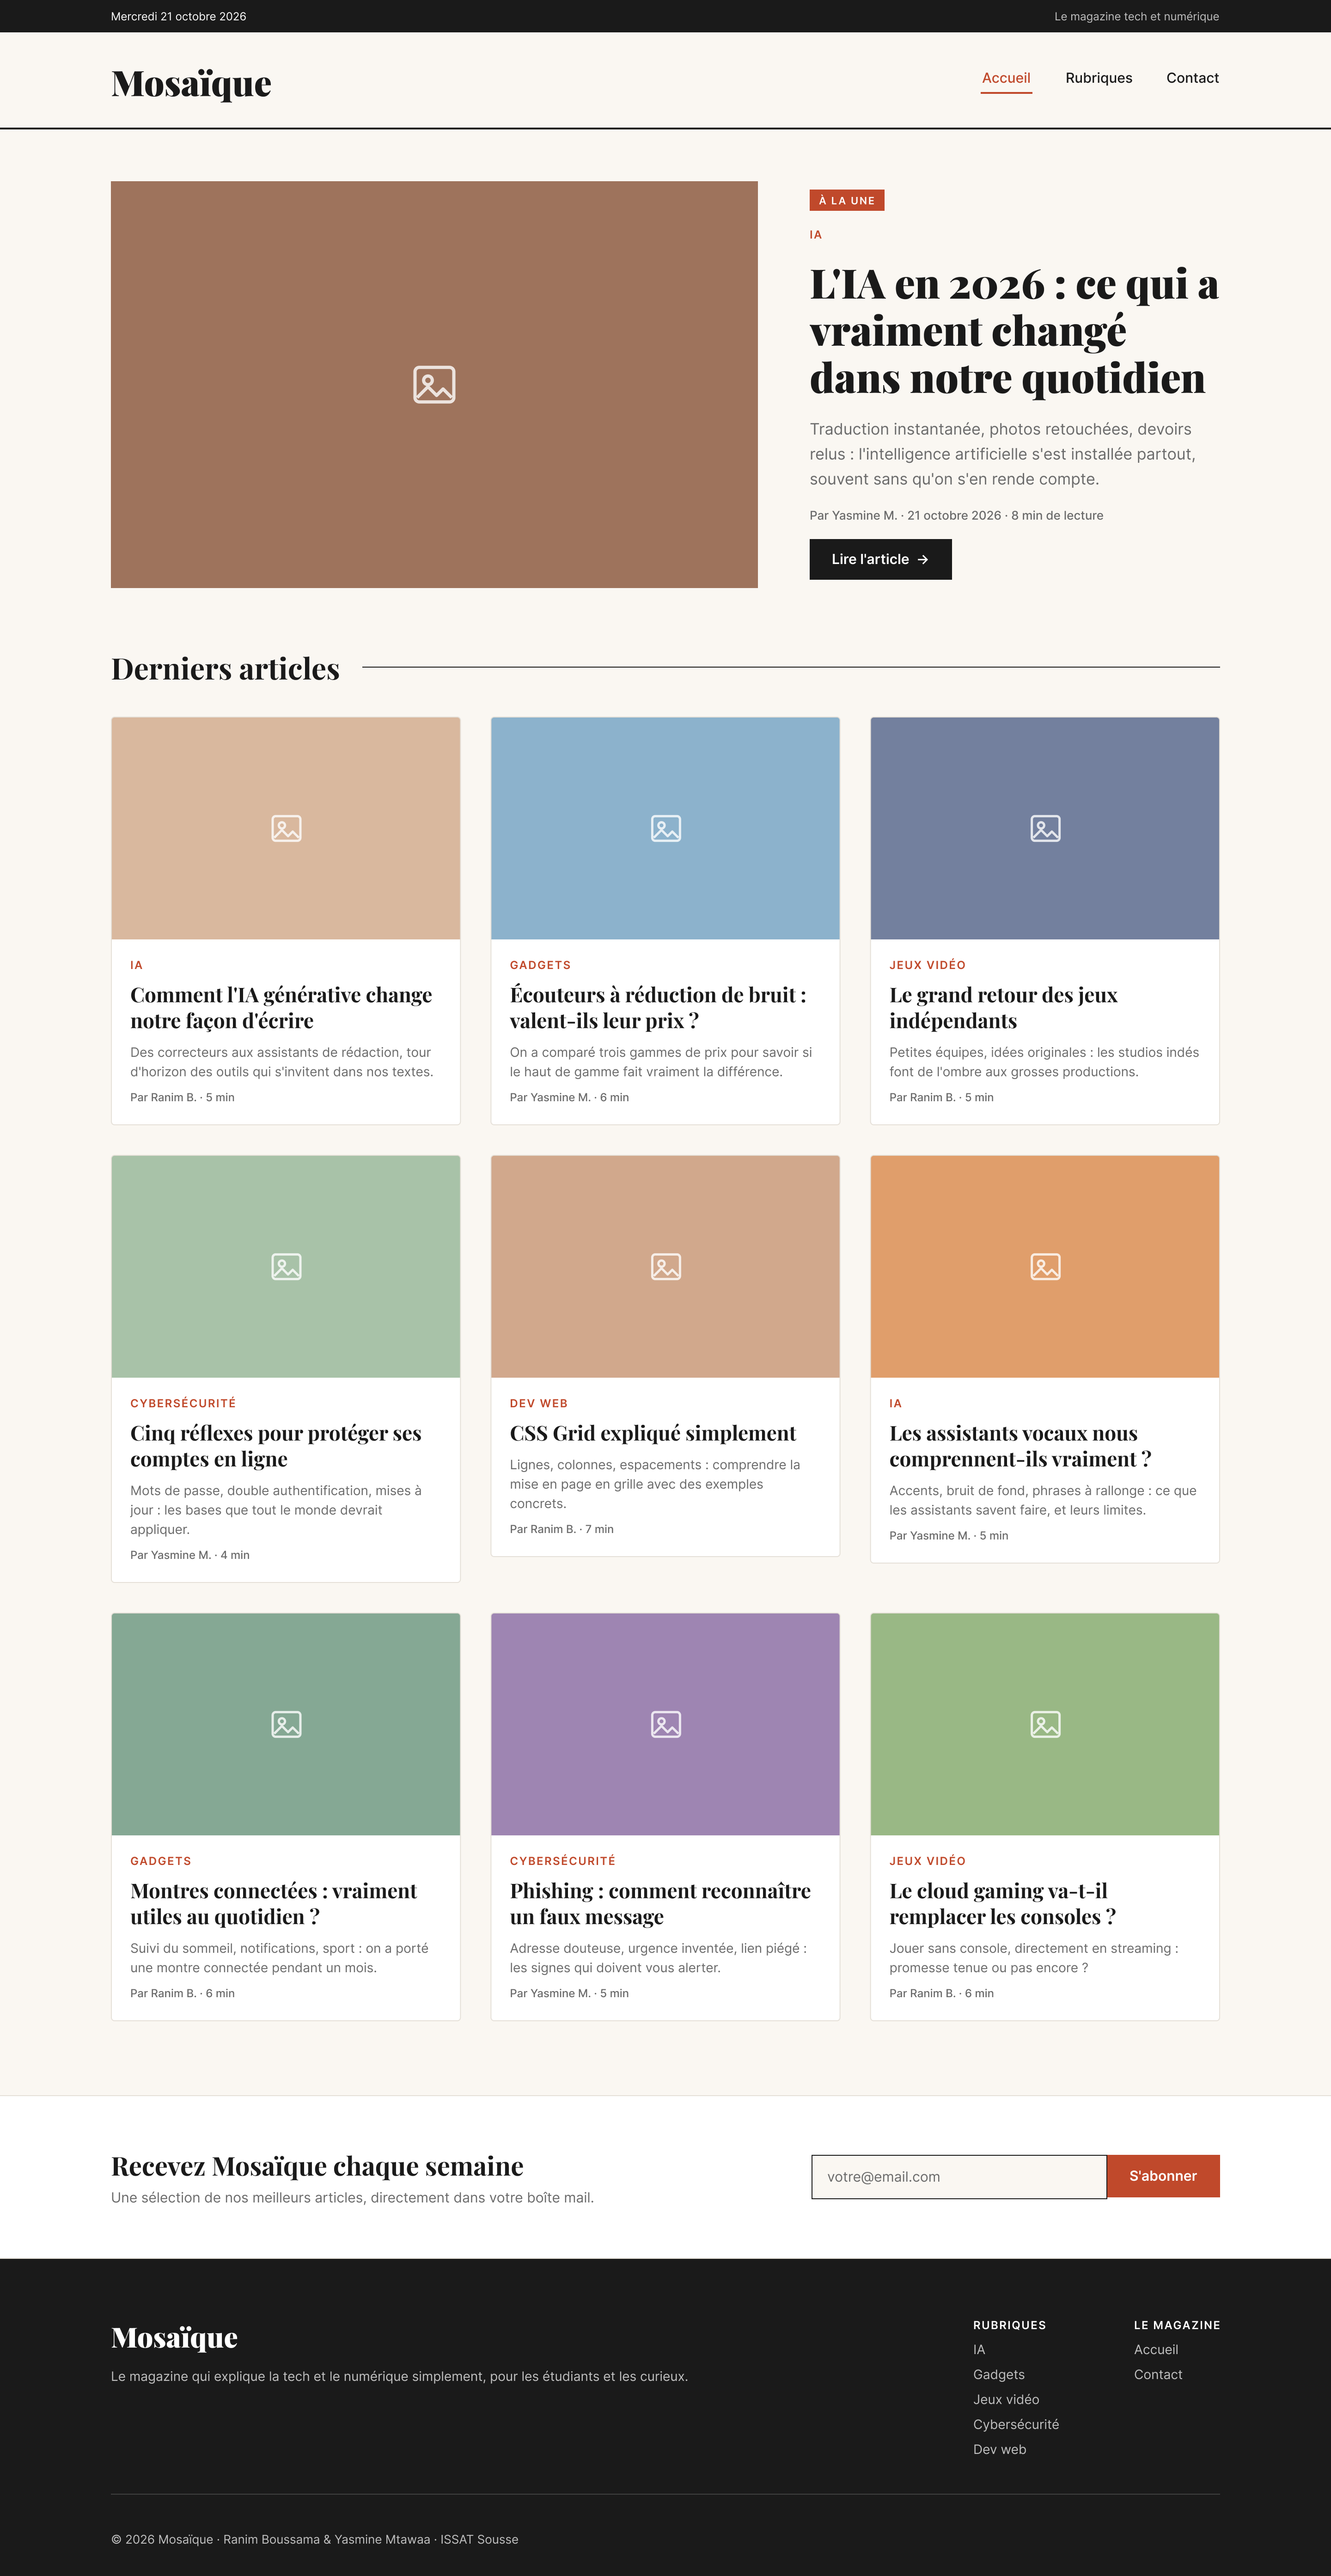
\includegraphics[width=\linewidth,height=0.62\textheight,keepaspectratio]{images/maquette-accueil.png}
    \caption{Page d'accueil : article à la une, grille de 9 articles,
      newsletter et pied de page}
  \end{subfigure}\hfill
  \begin{subfigure}[t]{0.45\textwidth}
    \centering
    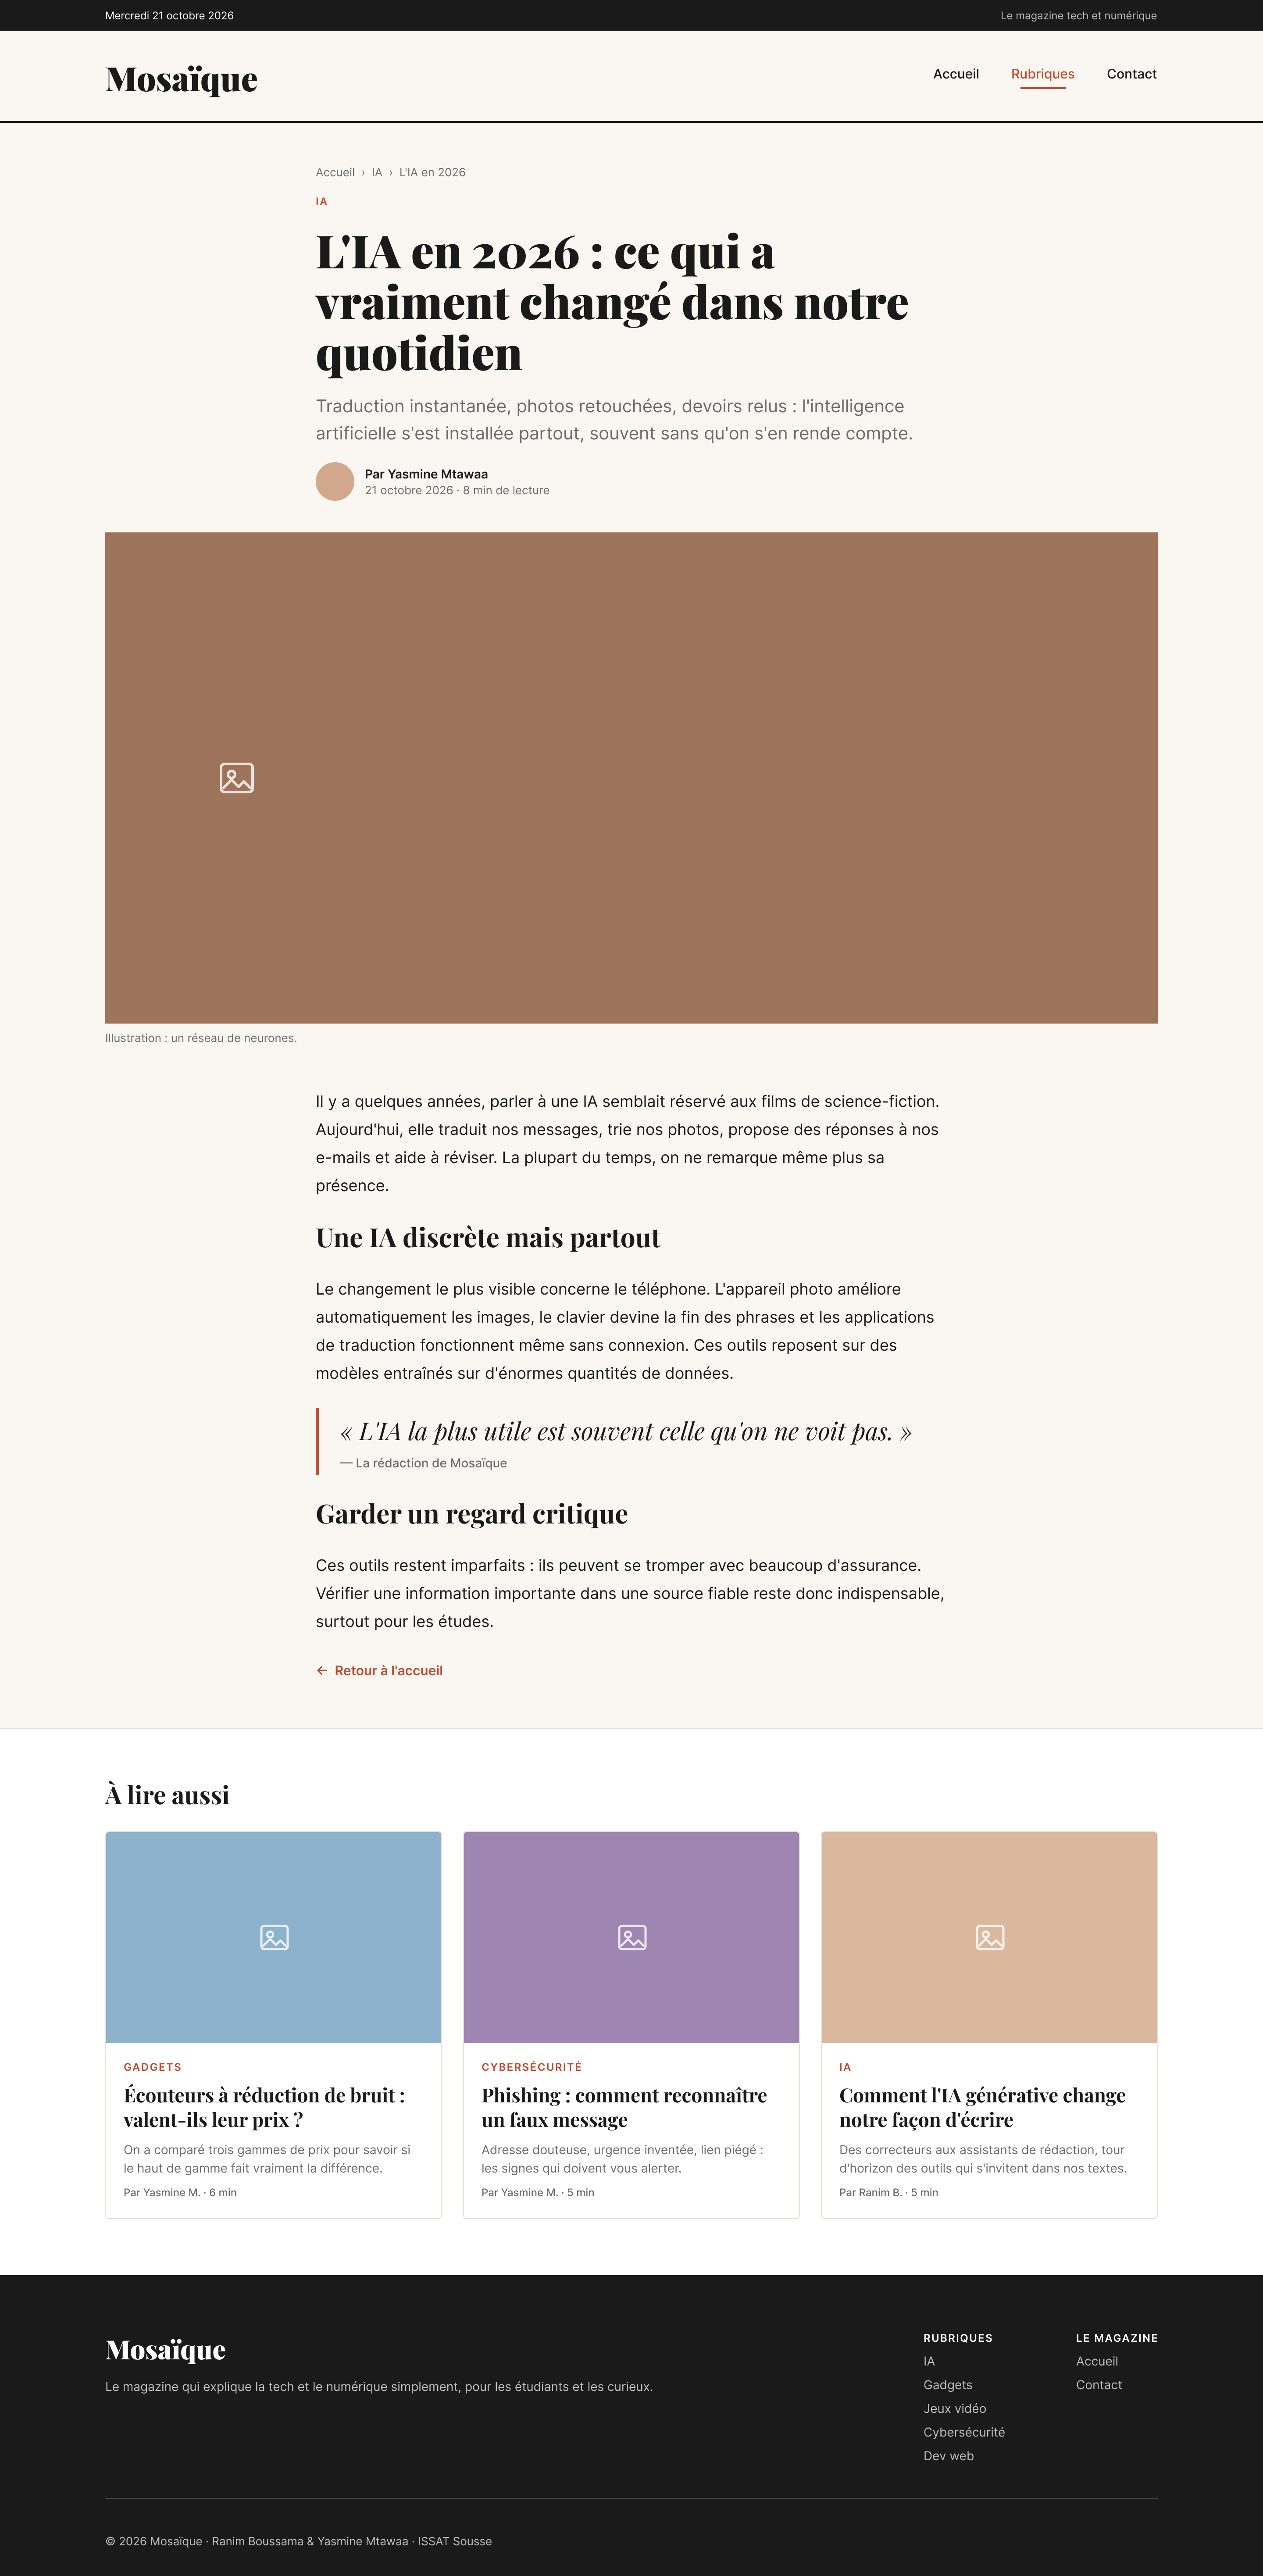
\includegraphics[width=\linewidth,height=0.62\textheight,keepaspectratio]{images/maquette-article.png}
    \caption{Page article : fil d'Ariane, en-tête, citation et section
      « À lire aussi »}
  \end{subfigure}
  \caption{Maquettes Figma (version desktop)}
\end{figure}

\subsection{Outils utilisés}

\begin{table}[H]
  \centering
  \small
  \begin{tabularx}{\textwidth}{>{\raggedright\arraybackslash}p{6cm}X}
    \toprule
    \textbf{Outil} & \textbf{Rôle} \\
    \midrule
    Figma & Charte graphique et maquettes des pages \\
    Visual Studio Code & Écriture du code HTML et CSS \\
    Extension Live Server & Aperçu du site en direct pendant le développement \\
    Google Chrome (outils de développement) & Tests du rendu et du mode responsive \\
    Google Fonts & Polices Playfair Display et Inter \\
    Validateurs W3C (HTML et CSS) & Vérification de la validité du code \\
    Git et GitHub & Partage du code et historique des versions à deux \\
    \bottomrule
  \end{tabularx}
  \caption{Outils utilisés}
\end{table}

% =========================================================
\section{Implémentation}

Cette partie présente les extraits de code les plus importants de la
semaine 1 et explique les choix faits pour répondre au cahier des charges.

\subsection{Variables CSS : la charte graphique dans le code}

Les couleurs et les polices de la charte sont déclarées une seule fois
sous forme de variables dans \code{:root}. Toutes les règles du site les
réutilisent avec \code{var()}. Si l'on veut changer une couleur, il suffit
de la modifier à un seul endroit.

\begin{lstlisting}[language=CSS]
:root {
  --encre: #1A1A1A;        /* titres, texte */
  --papier: #FAF7F2;       /* fond des pages */
  --blanc: #FFFFFF;        /* cartes */
  --terracotta: #C0492B;   /* accent, liens, catégories */
  --gris: #6B6B6B;         /* texte secondaire */
  --bordure: #E5E0D8;      /* séparateurs */
  --police-titre: "Playfair Display", Georgia, "Times New Roman", serif;
  --police-texte: "Inter", "Segoe UI", Arial, sans-serif;
}
\end{lstlisting}

\subsection{En-tête et navigation}

L'en-tête utilise les balises \code{<header>} et \code{<nav>}. Le lien de
la page courante porte la classe \code{is-active} et l'attribut
\code{aria-current="page"}, ce qui le met en couleur terracotta et
l'annonce aux lecteurs d'écran. Les cinq rubriques sont regroupées dans
un menu déroulant « Catégories ».

\begin{lstlisting}[language=HTML5]
<nav class="main-nav" aria-label="Navigation principale">
  <!-- Case cachée + label : menu burger sans JavaScript -->
  <input type="checkbox" id="menu-toggle" class="nav-toggle">
  <label for="menu-toggle" class="nav-burger">
    <span class="burger-lines" aria-hidden="true"></span>
    <span class="visually-hidden">Ouvrir le menu</span>
  </label>
  <ul class="nav-list">
    <li><a href="index.html" class="nav-link is-active" aria-current="page">Accueil</a></li>
    <!-- Menu déroulant des rubriques -->
    <li class="nav-dropdown">
      <button type="button" class="nav-link dropdown-toggle" aria-haspopup="true">Catégories</button>
      <ul class="dropdown-menu">
        <li><a href="pages/categorie-ia.html" class="dropdown-link">IA</a></li>
        <!-- ... autres rubriques ... -->
      </ul>
    </li>
    <li><a href="pages/contact.html" class="nav-link">Contact</a></li>
  </ul>
</nav>
\end{lstlisting}

\paragraph{Menu déroulant sans JavaScript.} Le sous-menu est caché par
défaut (\code{display: none}). Il s'affiche au survol de la souris grâce
à \code{:hover}, et aussi au clavier grâce à \code{:focus-within} : dès
que le bouton « Catégories » ou un lien du sous-menu reçoit le focus
(touche Tab), le menu reste ouvert.

\begin{lstlisting}[language=CSS]
.dropdown-menu {
  display: none;          /* caché par défaut */
  position: absolute;     /* placé sous « Catégories » */
  top: 100%;
  border-top: 2px solid var(--terracotta);
  box-shadow: var(--ombre);
}

.nav-dropdown:hover .dropdown-menu,
.nav-dropdown:focus-within .dropdown-menu {
  display: block;         /* ouvert au survol ou au clavier */
}
\end{lstlisting}

\paragraph{Menu burger sans JavaScript.} Comme JavaScript n'est pas encore
autorisé, le menu mobile repose sur une case à cocher cachée. Le
\code{<label>} dessine l'icône burger ; un clic dessus coche la case, et
le sélecteur \code{:checked} associé au sélecteur de frère \code{\~{}}
affiche le menu. Sur mobile, les rubriques ne sont plus dans un menu
flottant : elles sont listées directement sous « Catégories », avec un
léger retrait.

\begin{lstlisting}[language=CSS]
@media (max-width: 700px) {
  .nav-list {
    display: none;          /* menu caché par défaut sur mobile */
  }

  .nav-toggle:checked ~ .nav-list {
    display: flex;          /* affiché quand la case est cochée */
  }

  .dropdown-menu {
    display: block;         /* rubriques toujours visibles dans le menu */
    position: static;
  }
}
\end{lstlisting}

\subsection{Grille d'articles avec CSS Grid}

Chaque carte est un \code{<article>} entièrement cliquable, qui mène vers
la page de l'article. C'est ce qui simule la navigation entre les pages.

\begin{lstlisting}[language=HTML5]
<article class="card">
  <a href="pages/article-6.html" class="card-link">
    <div class="card-media">
      <img src="images/article-6.png" alt="Lignes de code HTML et CSS dans un éditeur" width="800" height="500">
    </div>
    <div class="card-body">
      <span class="tag tag-dev">Dev web</span>
      <h3 class="card-title">CSS Grid expliqué simplement</h3>
      <p class="card-excerpt">Lignes, colonnes, espacements : comprendre la mise en page en grille avec des exemples concrets.</p>
      <p class="card-meta">Par Ranim B., 7 min de lecture</p>
    </div>
  </a>
</article>
\end{lstlisting}

La grille est construite avec \code{display: grid} et trois colonnes de
même largeur (\code{1fr}). L'espace entre les cartes est géré par
\code{gap}, sans marges à calculer.

\begin{lstlisting}[language=CSS]
.grid {
  display: grid;
  grid-template-columns: repeat(3, 1fr); /* 3 colonnes sur ordinateur */
  gap: 28px;
}
\end{lstlisting}

\subsection{Effet zoom au survol}

Le cadre de l'image (\code{.card-media}) a \code{overflow: hidden} :
quand l'image grossit, ce qui dépasse est coupé et la carte garde sa
taille. Au survol, l'image passe à \code{scale(1.1)} avec une transition
de 0,5\,s, la carte reçoit une ombre et le titre devient terracotta, comme
sur la maquette Figma. L'effet marche aussi au clavier grâce à
\code{:focus-visible}.

\begin{lstlisting}[language=CSS]
.card-media {
  overflow: hidden;          /* coupe l'image qui grossit */
  aspect-ratio: 16 / 10;
}

.card-media img {
  object-fit: cover;
  transition: transform 0.5s ease;
}

.card-link:hover .card-media img,
.card-link:focus-visible .card-media img {
  transform: scale(1.1);     /* zoom de 10 % */
}

.card:hover {
  box-shadow: var(--ombre);
}
\end{lstlisting}

\subsection{Responsive design avec les media queries}

Le site s'adapte à plusieurs tailles d'écran. Le nombre de colonnes de la
grille change, et l'article à la une passe de deux colonnes à une seule.

\begin{table}[H]
  \centering
  \small
  \begin{tabularx}{\textwidth}{l l l X}
    \toprule
    \textbf{Écran} & \textbf{Largeur} & \textbf{Grille} & \textbf{Autres changements} \\
    \midrule
    Ordinateur & plus de 1024px & 3 colonnes & Menu horizontal, sous-menu « Catégories » au survol \\
    Tablette & 1024px et moins & 2 colonnes & Article à la une empilé, newsletter en colonne \\
    Mobile & 700px et moins & 2 colonnes & Menu burger, rubriques listées dans le menu, marges réduites \\
    Petit téléphone & 520px et moins & 1 colonne & --- \\
    \bottomrule
  \end{tabularx}
  \caption{Points de rupture (media queries)}
\end{table}

\begin{lstlisting}[language=CSS]
@media (max-width: 1024px) {
  .grid { grid-template-columns: repeat(2, 1fr); }
  .hero { grid-template-columns: 1fr; }
}

@media (max-width: 520px) {
  .grid { grid-template-columns: 1fr; }
}
\end{lstlisting}

Enfin, la règle \code{@media (prefers-reduced-motion: reduce)} désactive
les animations pour les personnes qui l'ont demandé dans les réglages de
leur système.

\subsection{Accessibilité}

Plusieurs détails rendent le site utilisable par tous : un lien « Aller
au contenu » visible seulement au clavier, un texte alternatif sur chaque
image, un contour terracotta visible au focus clavier, un menu déroulant
qui s'ouvre aussi au clavier, et la classe \code{.visually-hidden} pour
les textes destinés aux lecteurs d'écran (par exemple le titre
\code{<h1>} de l'accueil ou le libellé du champ newsletter).

% =========================================================
\clearpage
\section{Résultat final}

\subsection{Version ordinateur}

La page d'accueil reprend fidèlement la maquette Figma : bandeau noir,
logo en Playfair Display, article à la une sur deux colonnes, puis la
grille de neuf articles. Les vraies photos remplacent les blocs de couleur
de la maquette ; grâce à \code{object-fit: cover} et
\code{aspect-ratio}, elles ont toutes le même format, ce qui garde des
cartes alignées.

\begin{figure}[H]
  \centering
  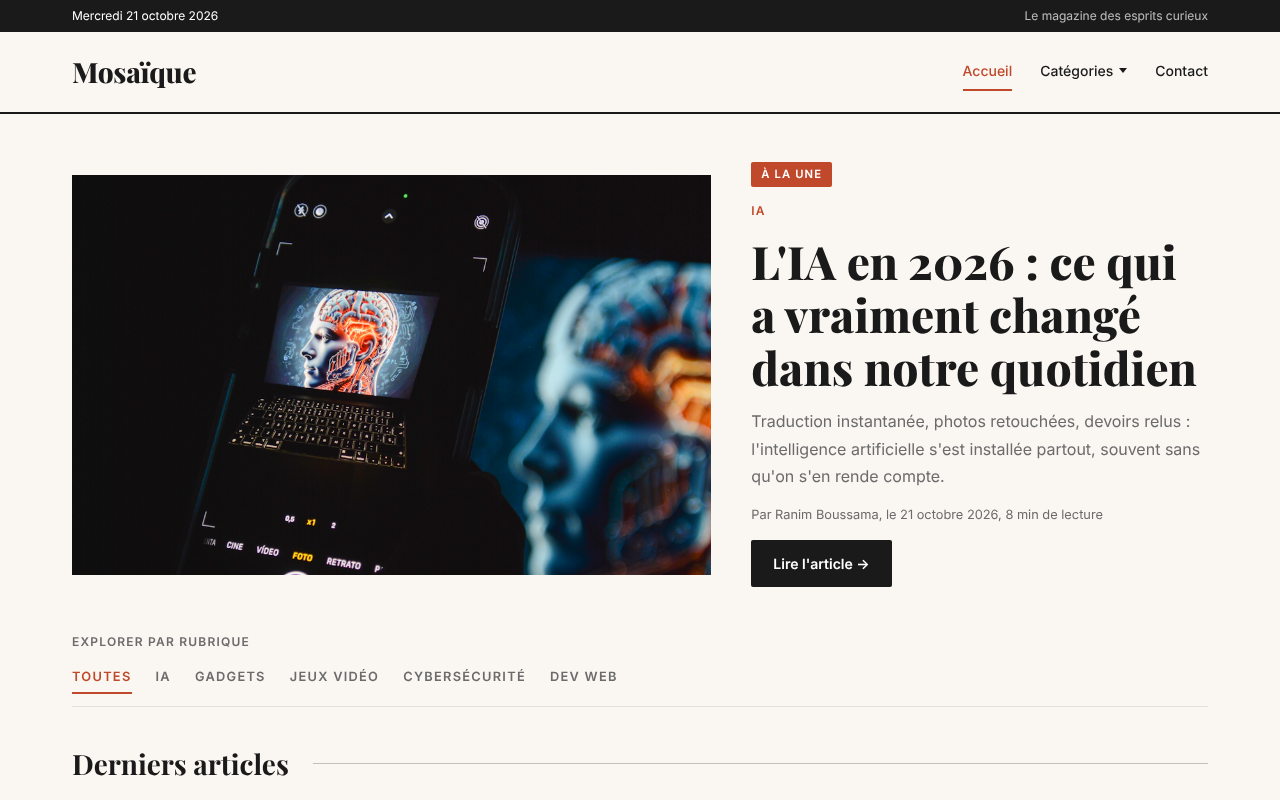
\includegraphics[width=\textwidth]{images/accueil-desktop-haut.png}
  \caption{Haut de la page d'accueil sur ordinateur (1280px)}
\end{figure}

\begin{figure}[H]
  \centering
  \begin{subfigure}[t]{0.48\textwidth}
    \centering
    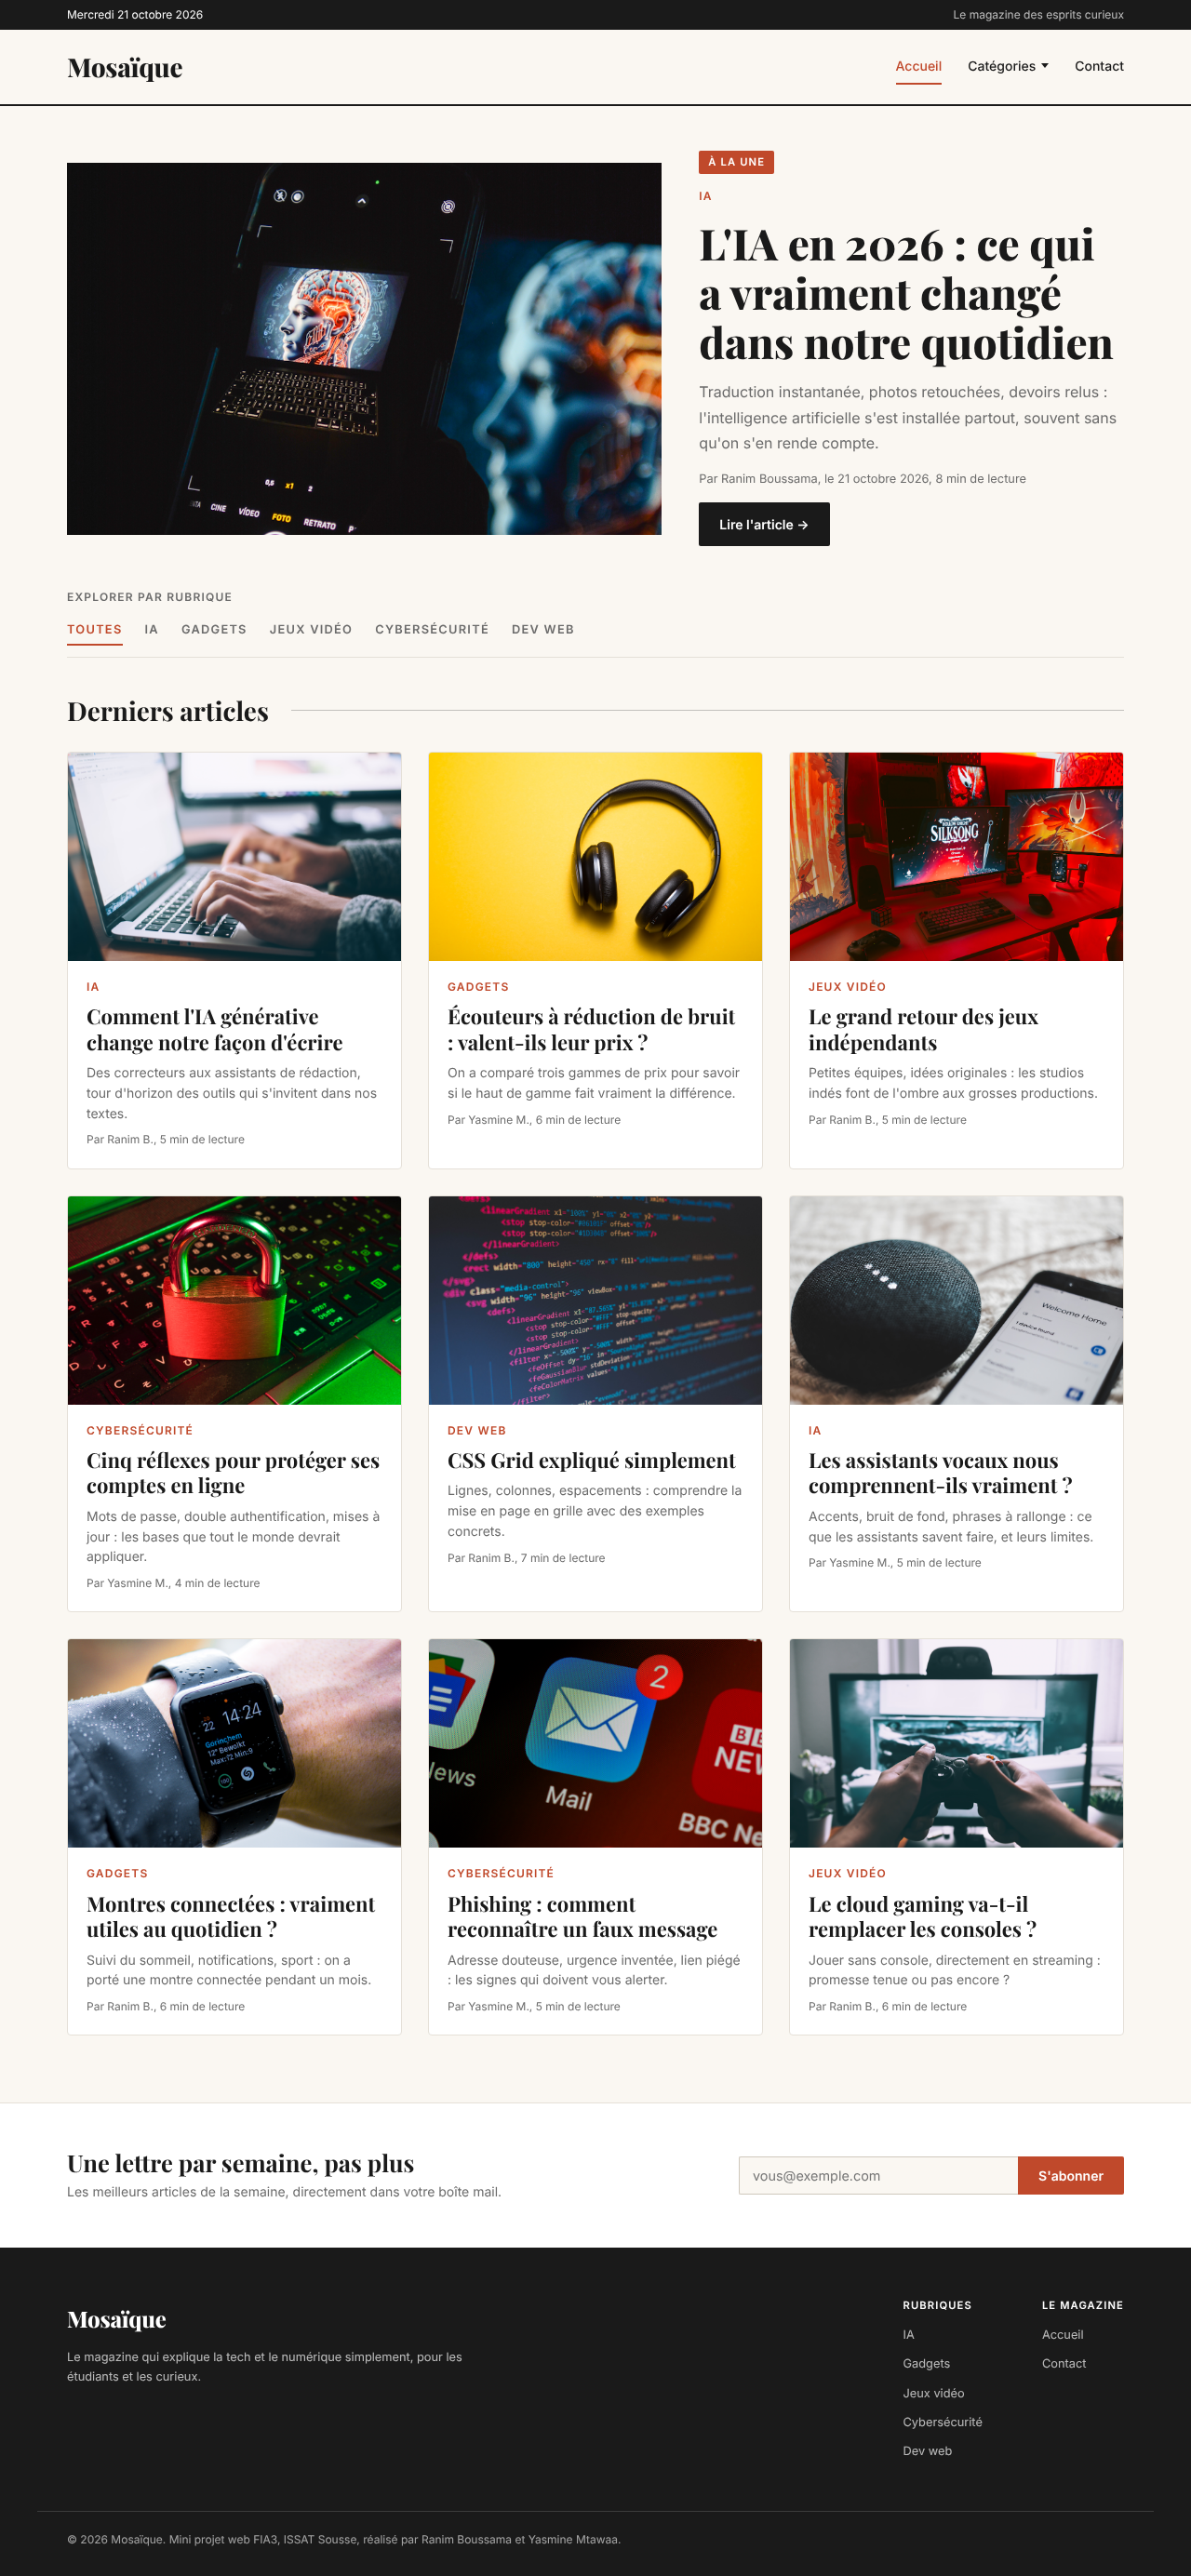
\includegraphics[width=\linewidth,height=0.6\textheight,keepaspectratio]{images/accueil-desktop.png}
    \caption{Page d'accueil complète}
  \end{subfigure}\hfill
  \begin{subfigure}[t]{0.48\textwidth}
    \centering
    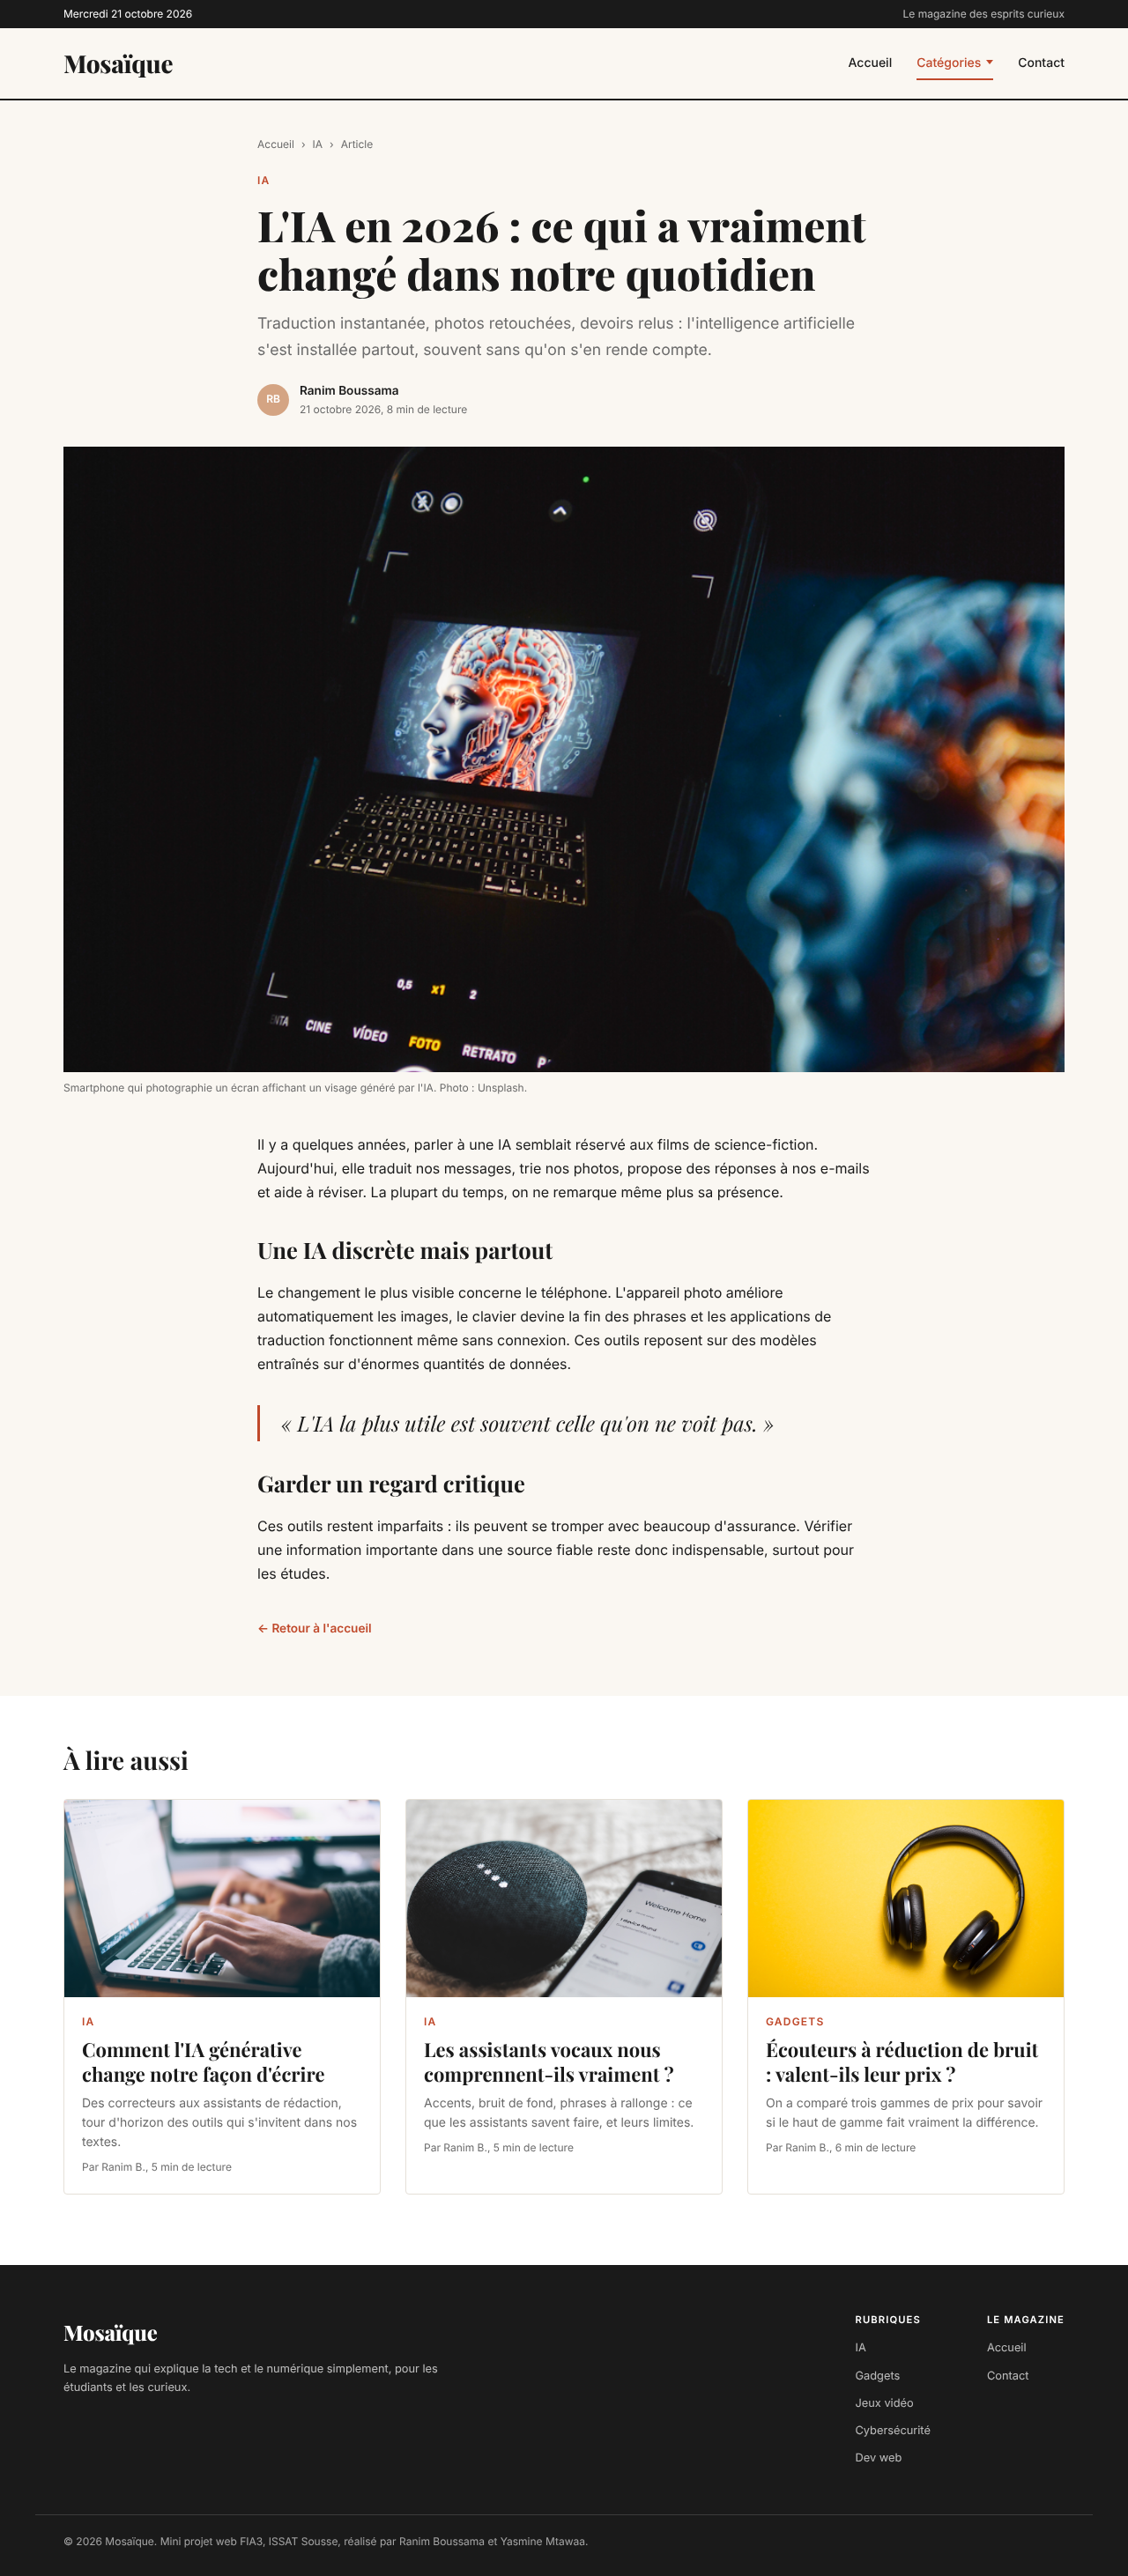
\includegraphics[width=\linewidth,height=0.6\textheight,keepaspectratio]{images/article-desktop.png}
    \caption{Page article complète}
  \end{subfigure}
  \caption{Pages complètes sur ordinateur}
\end{figure}

La figure~\ref{fig:survol} montre l'effet demandé par le sujet : la carte
survolée (à gauche) a son image agrandie, une ombre et un titre
terracotta, alors que la carte voisine reste dans son état normal. Le
menu déroulant « Catégories » (figure~\ref{fig:dropdown}) reprend les
mêmes codes : filet terracotta et ombre légère.

\begin{figure}[H]
  \centering
  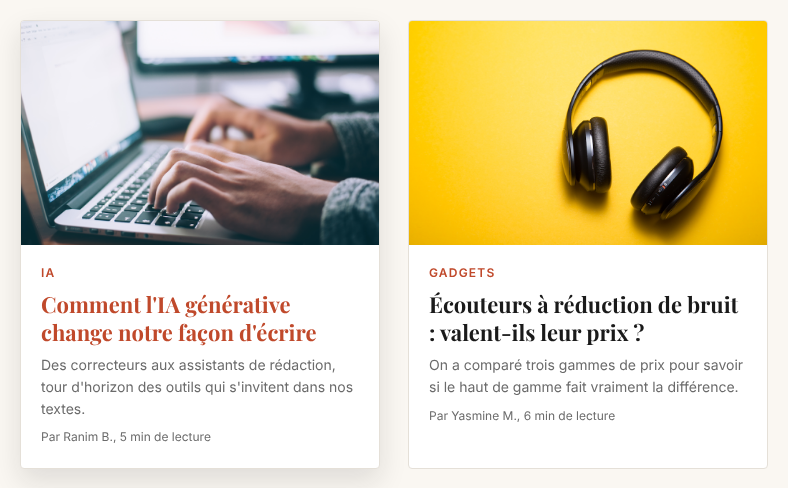
\includegraphics[width=0.75\textwidth]{images/carte-survol.png}
  \caption{Carte au survol (à gauche) et carte normale (à droite)}
  \label{fig:survol}
\end{figure}

\begin{figure}[H]
  \centering
  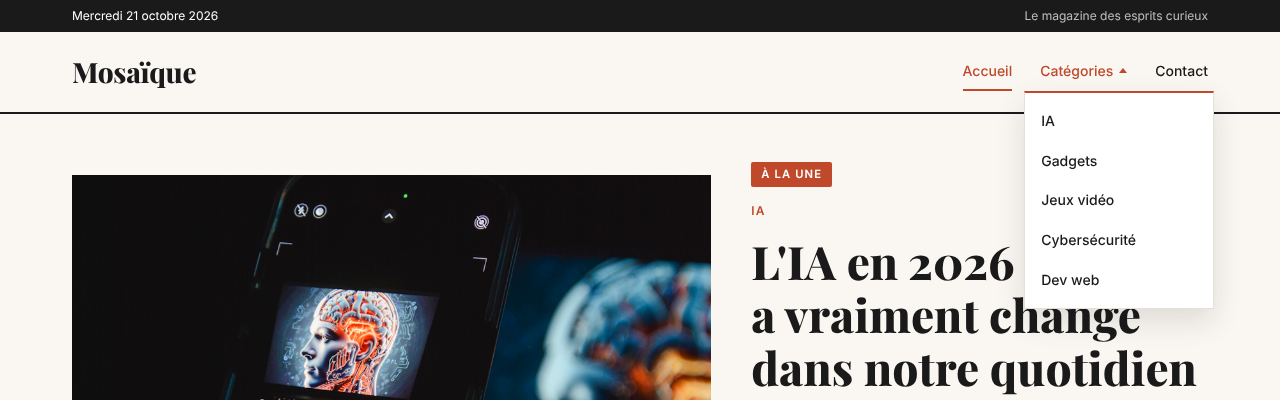
\includegraphics[width=\textwidth]{images/menu-deroulant.png}
  \caption{Menu déroulant « Catégories » ouvert au survol}
  \label{fig:dropdown}
\end{figure}

\begin{figure}[H]
  \centering
  \begin{subfigure}[t]{0.49\textwidth}
    \centering
    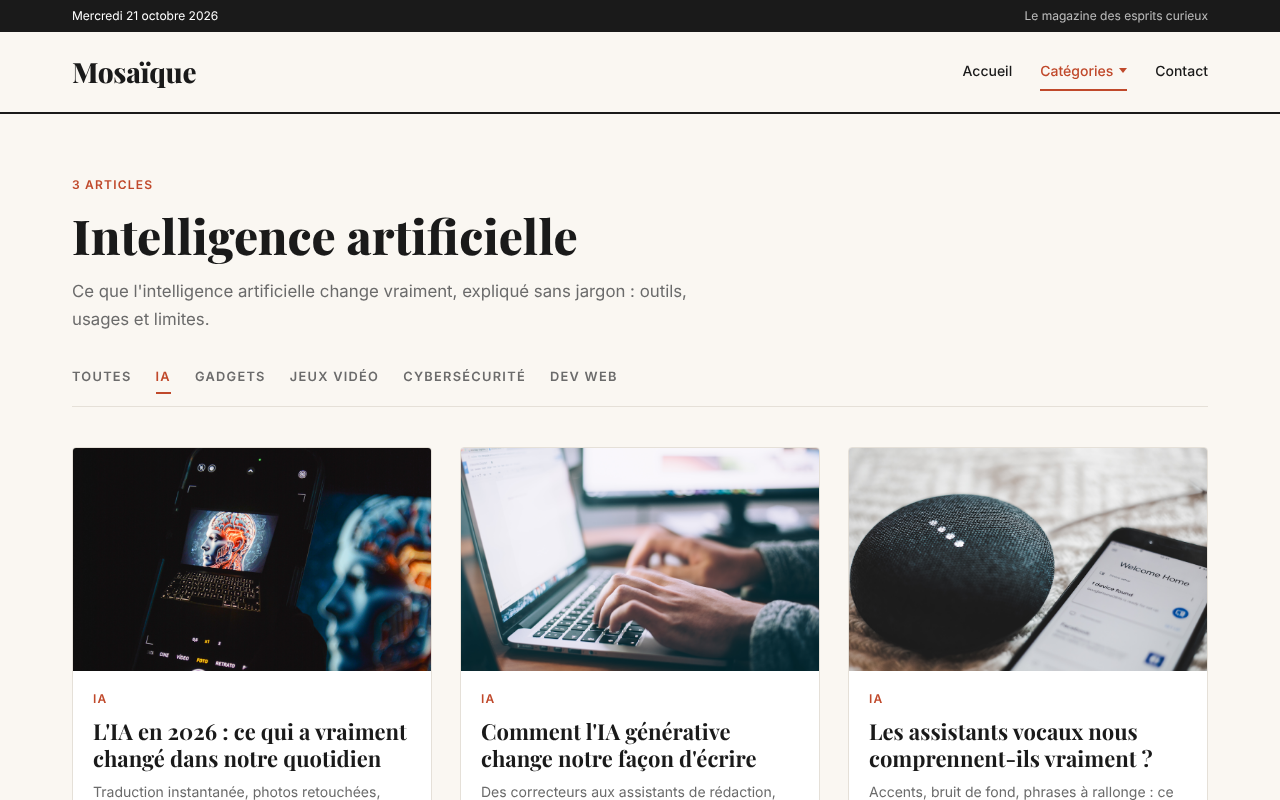
\includegraphics[width=\textwidth]{images/rubrique-desktop.png}
    \caption{Page rubrique (IA)}
  \end{subfigure}\hfill
  \begin{subfigure}[t]{0.49\textwidth}
    \centering
    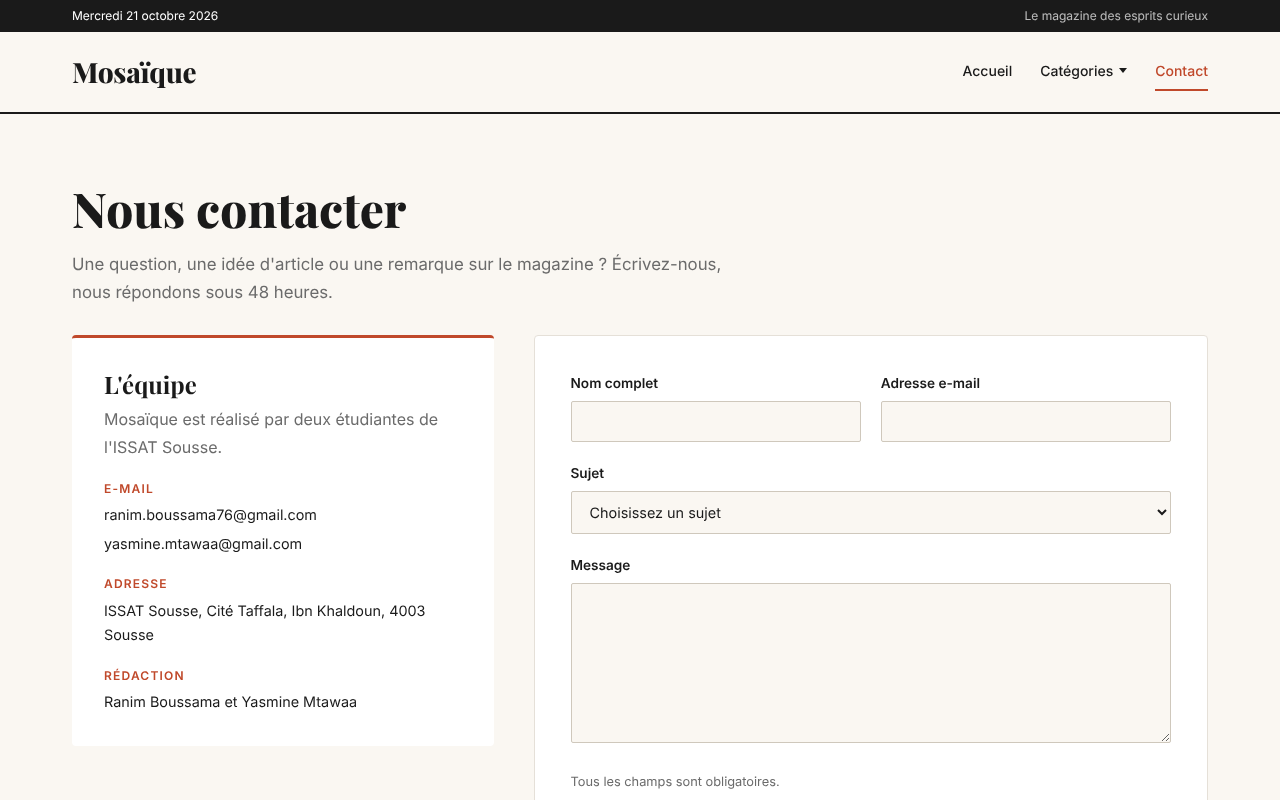
\includegraphics[width=\textwidth]{images/contact-desktop.png}
    \caption{Page contact}
  \end{subfigure}
  \caption{Pages rubrique et contact}
\end{figure}

\subsection{Versions tablette et mobile}

Sur tablette, l'article à la une passe au-dessus de son texte et la
grille passe à deux colonnes. Sur mobile, la navigation se replie dans le
menu burger ; une fois ouvert, il liste directement les cinq rubriques
sous « Catégories ». Sur un petit téléphone, les cartes s'affichent sur
une seule colonne.

\begin{figure}[H]
  \centering
  \begin{subfigure}[t]{0.36\textwidth}
    \centering
    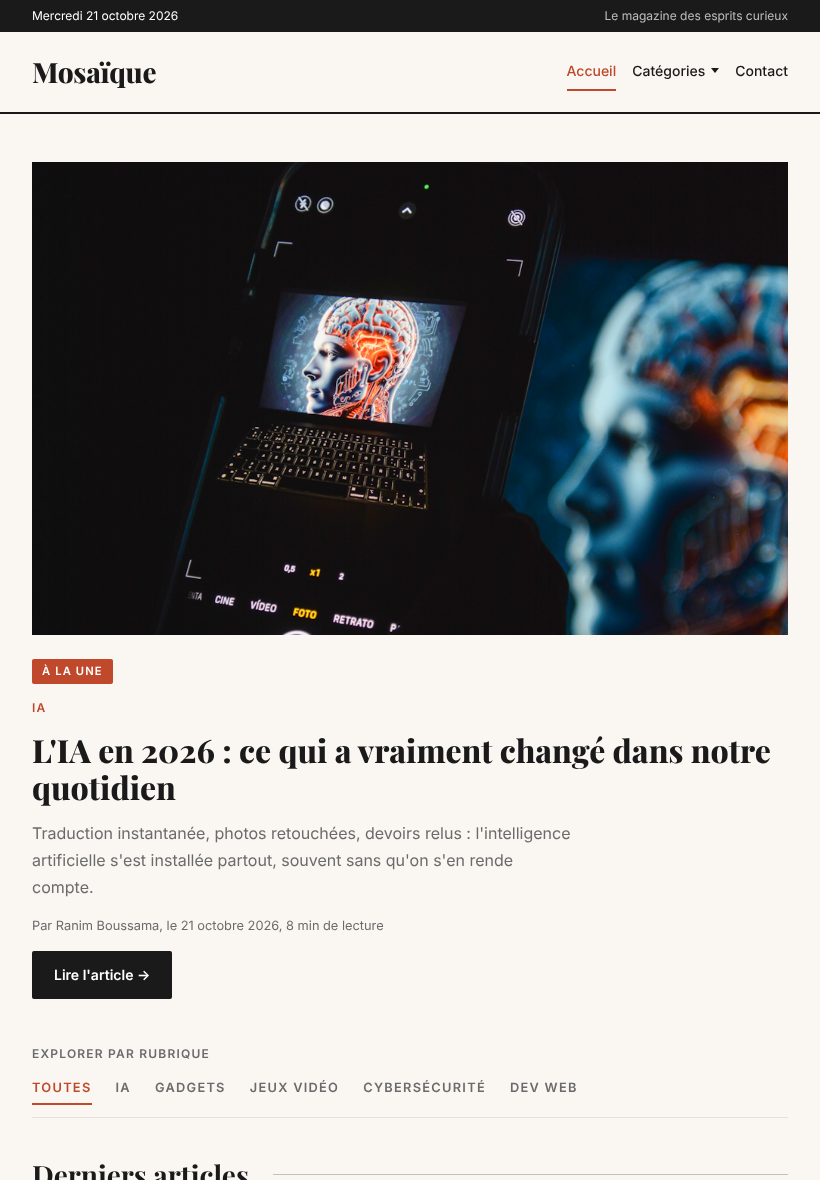
\includegraphics[height=7.5cm]{images/accueil-tablette.png}
    \caption{Tablette (820px)}
  \end{subfigure}\hfill
  \begin{subfigure}[t]{0.3\textwidth}
    \centering
    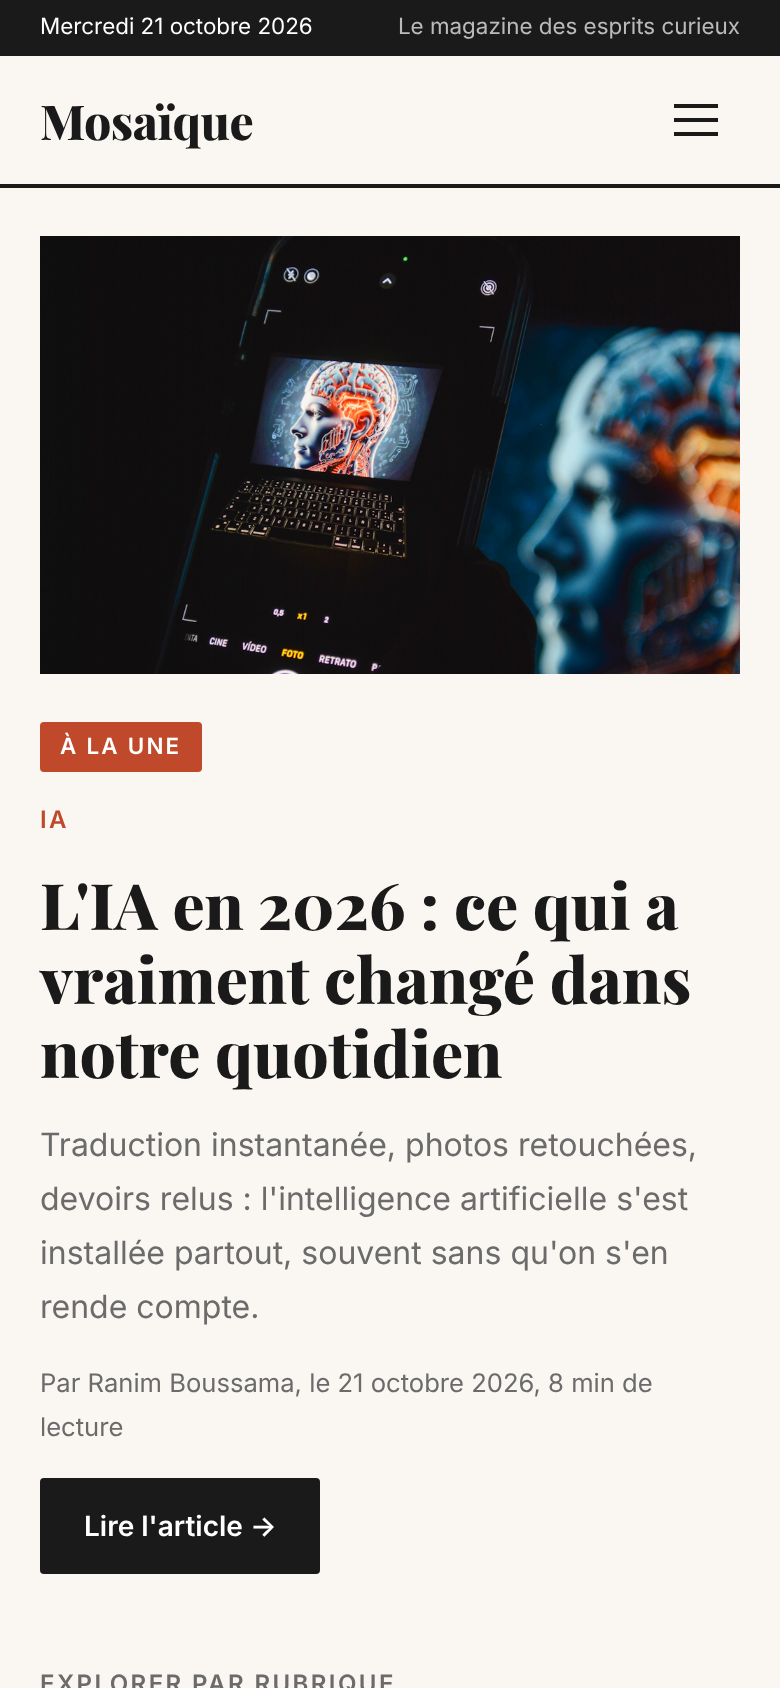
\includegraphics[height=7.5cm]{images/accueil-mobile.png}
    \caption{Mobile (390px)}
  \end{subfigure}\hfill
  \begin{subfigure}[t]{0.3\textwidth}
    \centering
    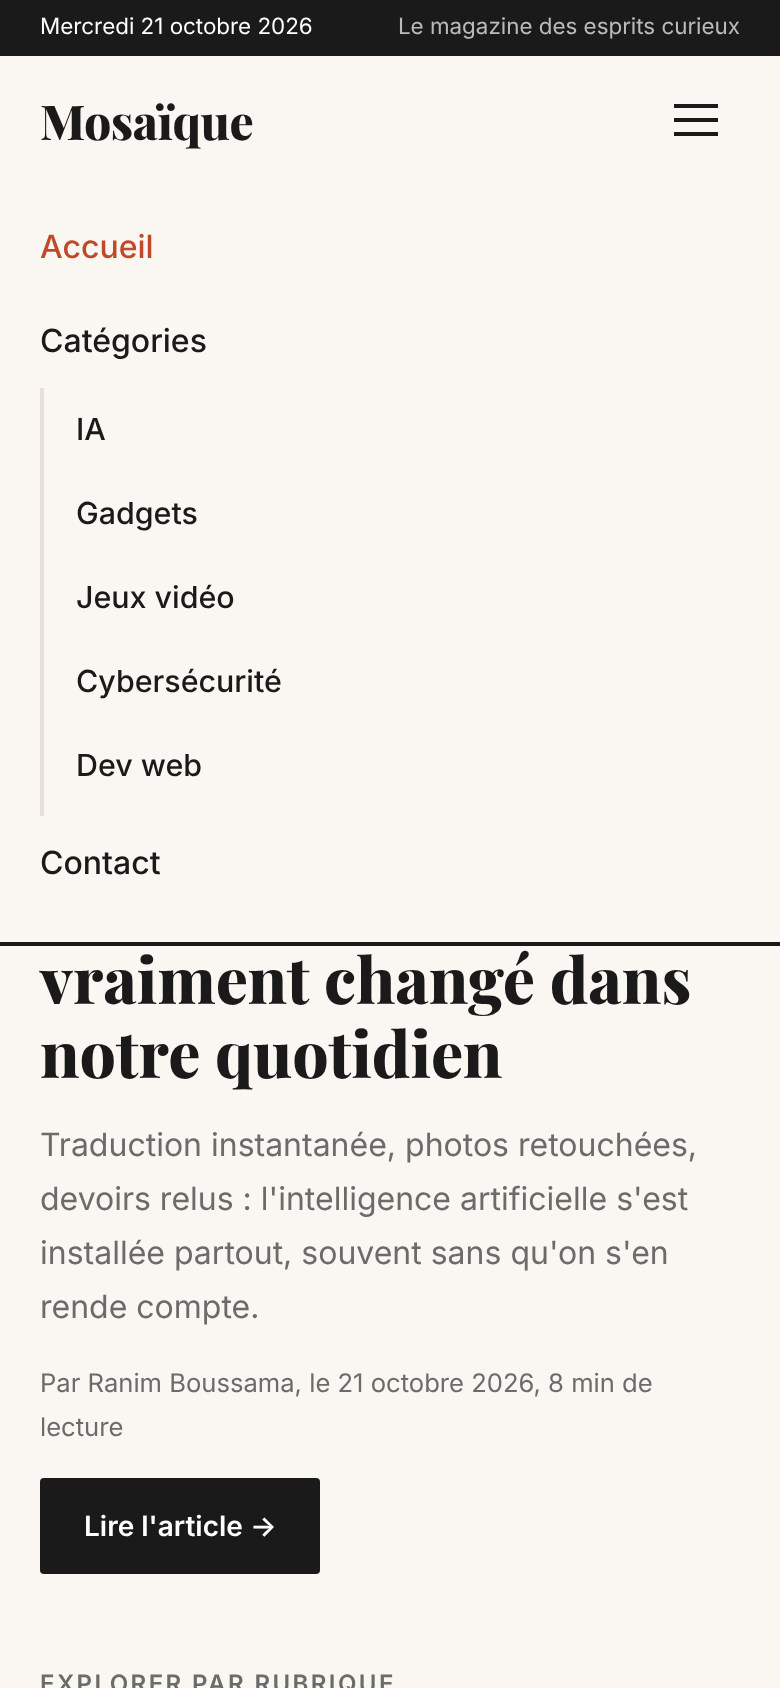
\includegraphics[height=7.5cm]{images/menu-mobile.png}
    \caption{Menu burger ouvert}
  \end{subfigure}
  \caption{Rendu responsive}
\end{figure}

\subsection{Commentaire du rendu}

\begin{itemize}
  \item \textbf{Mise en page} : la grille CSS garde des cartes de même
    largeur et bien alignées, quel que soit le nombre de lignes de texte.
  \item \textbf{Responsive} : le site reste lisible de 1280px jusqu'à
    390px de large, sans défilement horizontal.
  \item \textbf{Cohérence visuelle} : toutes les pages partagent le même
    en-tête, le même pied de page et la même feuille de style, et
    respectent la charte (une seule couleur d'accent, deux polices).
  \item \textbf{Navigation} : toutes les cartes, les rubriques, le fil
    d'Ariane et le lien « Retour à l'accueil » mènent à de vraies pages ;
    aucun lien n'est vide.
\end{itemize}

\subsection{Liens du projet}

\begin{tcolorbox}[
    enhanced,
    colback=papier,
    colframe=bordure,
    boxrule=0.6pt,
    arc=1mm,
    borderline west={3pt}{0pt}{terracotta},  % filet terracotta, comme les citations du site
    left=6mm, right=6mm, top=5mm, bottom=5mm
]
  % --- Site déployé ---
  \etiquette{\faGlobe\ Site web déployé}\\[1mm]
  {\Large\bfseries\color{encre} Mosaïque est en ligne}\\[1mm]
  {\color{gris} Le magazine est consultable depuis un ordinateur, une
  tablette ou un téléphone.}\\[3mm]
  \bouton{https://mini-magazine-mosaique.vercel.app/}{Accéder au site $\rightarrow$}%
  \hspace{3mm}{\small\color{gris}\url{https://mini-magazine-mosaique.vercel.app/}}

  \vspace{3mm}
  \noindent{\color{bordure}\rule{\linewidth}{0.6pt}}\\[3mm]
  % --- Dépôts GitHub ---
  \depot{Dépôt GitHub 1}{Ranim Boussama}{ranimboussama76-eng}{mini-magazine-mosaique}%
  \hfill
  \depot{Dépôt GitHub 2}{Yasmine Mtawaa}{yasmine-mtawaa}{mini-magazine-mosaique}
\end{tcolorbox}

\subsection{Validation W3C}

Le sujet impose la validation du code par le W3C. Nous avons vérifié la
page d'accueil avec le validateur HTML (Nu Html Checker) et la feuille de
style avec le validateur CSS (CSS niveau 3 + SVG).

\begin{itemize}
  \item \textbf{HTML} : \code{index.html} ne contient aucune erreur et
    aucun avertissement (figure~\ref{fig:w3c-html}).
  \item \textbf{CSS} : \code{style.css} ne contient aucune erreur
    (figure~\ref{fig:w3c-css}). Le validateur affiche 12 avertissements,
    qui ne sont pas des erreurs et n'empêchent pas la validation.
\end{itemize}

\begin{figure}[H]
  \centering
  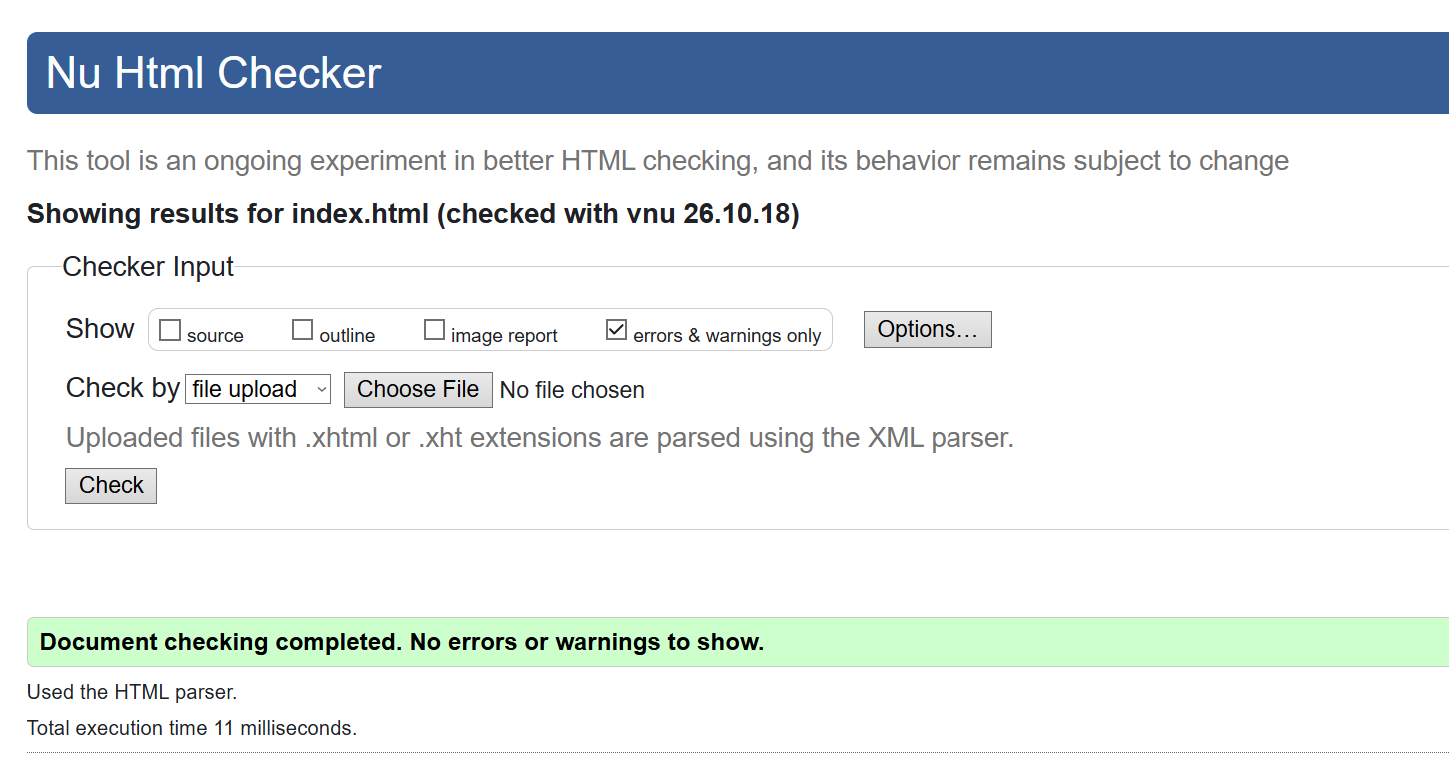
\includegraphics[width=0.85\textwidth]{images/validation-html.png}
  \caption{Validation HTML de \code{index.html} : aucune erreur ni
    avertissement}
  \label{fig:w3c-html}
\end{figure}

\begin{figure}[H]
  \centering
  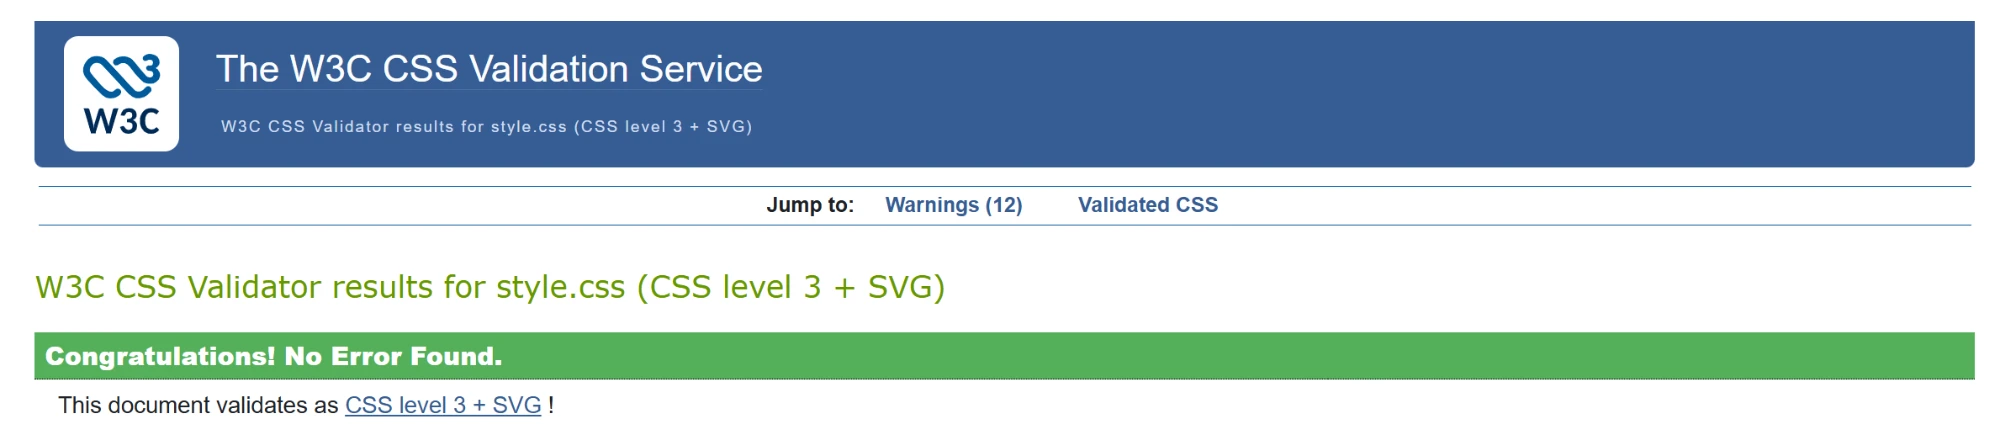
\includegraphics[width=\textwidth]{images/validation-css.png}
  \caption{Validation CSS de \code{style.css} : aucune erreur}
  \label{fig:w3c-css}
\end{figure}

% =========================================================
\section{Difficultés rencontrées et solutions}

\begin{itemize}[leftmargin=*]
  \item \textbf{Menu mobile sans JavaScript.} Ouvrir et fermer un menu
    demande normalement du JavaScript, interdit en semaine 1.
    \textit{Solution :} une case à cocher cachée, reliée à un
    \code{<label>} qui dessine le burger ; le sélecteur
    \code{:checked \~{} .nav-list} affiche le menu.

  \item \textbf{Menu déroulant utilisable au clavier.} Avec seulement
    \code{:hover}, le sous-menu « Catégories » se refermait dès qu'on
    naviguait avec la touche Tab. \textit{Solution :} ajouter
    \code{:focus-within}, qui garde le menu ouvert tant qu'un de ses
    éléments a le focus. Sur mobile, où le survol n'existe pas, les
    rubriques sont affichées directement dans le menu burger.

  \item \textbf{Trop de liens dans la barre de navigation.} Avec les cinq
    rubriques plus Accueil et Contact, la barre débordait sur tablette.
    \textit{Solution :} regrouper les rubriques dans le menu déroulant
    « Catégories », comme sur la maquette.

  \item \textbf{Image qui dépasse de la carte au zoom.} Avec
    \code{scale(1.1)}, l'image agrandie sortait de son cadre.
    \textit{Solution :} \code{overflow: hidden} sur le conteneur
    \code{.card-media}.

  \item \textbf{Photos de tailles différentes.} Les images n'avaient pas
    toutes le même format, et les cartes n'étaient pas alignées.
    \textit{Solution :} un cadre fixe avec \code{aspect-ratio: 16 / 10} et
    \code{object-fit: cover}, qui recadre chaque photo sans la déformer.

  \item \textbf{Marges écrasées sur mobile.} Une règle \code{padding} dans
    la media query mobile annulait les marges haut et bas des sections.
    \textit{Solution :} ne modifier que \code{padding-left} et
    \code{padding-right}.

  \item \textbf{Travail à deux sur le même code.} \textit{Solution :} un
    dépôt GitHub commun, avec un fichier \code{.gitignore} et des messages
    de commit clairs pour suivre les changements.
\end{itemize}

% =========================================================
\section{Conclusion}

Cette première étape nous a permis de consolider nos connaissances en
HTML et CSS : structurer une page avec des balises sémantiques, organiser
une feuille de style avec des variables, construire une mise en page avec
CSS Grid et Flexbox, et adapter le site à toutes les tailles d'écran avec
les media queries. Nous avons aussi découvert qu'on peut obtenir beaucoup
d'interactivité en CSS pur (menu burger, menu déroulant, effets de
survol), et l'importance de l'accessibilité.

Le projet n'est pas terminé : il servira de base aux deux semaines
suivantes. En semaine 2, nous ajouterons JavaScript pour valider les
formulaires de newsletter et de contact et rendre l'interface plus
interactive. En semaine 3, PHP permettra de traiter ces formulaires côté
serveur.

% =========================================================
\clearpage
\section{Annexes}

\subsection{Ressources et documentation utilisées}

\begin{itemize}
  \item MDN Web Docs (HTML, CSS Grid, Flexbox, media queries) :
    \url{https://developer.mozilla.org/fr/}
  \item Validateur HTML du W3C : \url{https://validator.w3.org/}
  \item Validateur CSS du W3C : \url{https://jigsaw.w3.org/css-validator/}
  \item Google Fonts (Playfair Display, Inter) : \url{https://fonts.google.com/}
  \item Photos des articles : \url{https://unsplash.com/}
\end{itemize}

\subsection{Code complet : index.html}
\codefile{language=HTML5,basicstyle=\ttfamily\scriptsize}{index.html}{../index.html}

\subsection{Code complet : css/style.css}
\codefile{language=CSS,basicstyle=\ttfamily\scriptsize}{style.css}{../css/style.css}

\end{document}
